\documentclass[10pt,twocolumn,letterpaper]{article}

\usepackage{cvpr}
\usepackage{times}
\usepackage{epsfig}
\usepackage{graphicx}
\usepackage{amsmath}
\usepackage{amssymb}
\usepackage{float}

% Include other packages here, before hyperref.

% If you comment hyperref and then uncomment it, you should delete
% egpaper.aux before re-running latex.  (Or just hit 'q' on the first latex
% run, let it finish, and you should be clear).
\usepackage[breaklinks=true,bookmarks=false]{hyperref}

\cvprfinalcopy % *** Uncomment this line for the final submission

\def\cvprPaperID{****} % *** Enter the CVPR Paper ID here
\def\httilde{\mbox{\tt\raisebox{-.5ex}{\symbol{126}}}}

% Pages are numbered in submission mode, and unnumbered in camera-ready
%\ifcvprfinal\pagestyle{empty}\fi
\setcounter{page}{1}
\begin{document}

%%%%%%%%% TITLE
\title{Instance Segmentation for Urban Street Scenes}

\author{Francesco Bari\\
{\tt\small francesco.bari.2@studenti.unipd.it}
% For a paper whose authors are all at the same institution,
% omit the following lines up until the closing ``}''.
% Additional authors and addresses can be added with ``\and'',
% just like the second author.
% To save space, use either the email address or home page, not both
\and
Eleonora Signor\\
{\tt\small eleonora.signor@studenti.unipd.it}
}

\maketitle
%\thispagestyle{empty}

%%%%%%%%% ABSTRACT
\begin{abstract}
In this report we compared different existing instance segmentation techniques, on the specific task of \textit{Urban Street Scenes}. Our interest in the topic was born out of the fact that the segmentation of instances is one of the fundamental tasks of the vision, however it is still complex and not fully explored.
%In questo lavoro abbiamo confrontato differenti tecniche di instance segmentation, gi\`a esistenti, sul task specifico di \textit{Urban Street Scenes}. Il nostro interesse verso il topic \`e nato dal fatto che la segmentazione delle istanze \`e uno dei compiti fondamentali della visione, tuttavia si presenta ancora complesso e non del tutto esplorato. 
%Esistono differenti approcci di instance segmentation, di seguito ne presentiamo una sottoparte, valutandone accuracy e performance su dataset multicategoriali e rivolti a quantificare la robustezza di un algoritmo.
\end{abstract}

%%%%%%%%% BODY TEXT
\section{Introduction}
Image segmentation is the process of separating an image into several segments,  in which each pixel is associated with an object type. There are two types of image segmentation: semantic segmentation and instance segmentation. The first marks objects of the same type with the equal class label; the second marks objects of the same type and belonging to distinct entities with different class labels. The idea we tried to develop was to compare different instance segmentation methods. The first technique we studied was Mask R-CNN~\cite{Authors1_maskrcnn}, a two-stage approach. We chose this one in the light of the positive feedback it has received from the world of vision research, due to its conceptually simple and general framework,  characterised by efficient image object detection, and the simultaneous generation of a high quality segmentation mask for each instance. The technique we decided to contrast with Mask R-CNN was BlendMask~\cite{Authors2_BlendMask}. Instead, this is a one-stage technique that has been shown to outperform Mask R-CNN both in terms of mask prediction and training time, on the MSCOCO 2017~\cite{Authors3_MSCOCO} and LVIS~\cite{Authors4_LVIS} datasets. We were interested in verifying whether this also applied to datasets, such as \textit{Cityscapes}~\cite{cityscapes} and \textit{WildDash}~\cite{wildDash}, belonging to the specific topic of \textit{Urban Street Scenes},  featuring images from the streets around the world, with many difficult scenarios. Some of the aspects we tested involved backbone changes, depth of the ResNet~\cite{Authors5_ResNet} and number of frozen layers.  The results obtained confirmed what had already been announced in previous works, generalising BlendMask as one of the most promising staged approaches. At the end of our work and in order not to limit our analysis, we also made some considerations on other instance segmentation techniques, such as SOLOv2~\cite{Authors6_SOLOv2} and Deep Snake~\cite{Authors7_deepsnake}.
%La segmentazione dell'immagine \`e il processo di separazione di questa in pi\`u segmenti, in cui ciascun pixel viene associato a un tipo di oggetto. Esistono due tipologie di segmentazione dell'immagine: la segmentazione semantica e la segmentazione d'instanza. La prima contrassegna oggetti dello stesso tipo con la medesima etichetta di classe; la seconda contrassegna oggetti dello stesso tipo e appartenenti a entit\`a distinte con etichette di classe differenti. L'idea che abbiamo cercato di sviluppare ha riguardato il confronto di diverse metodoligie di instance segmentation. La prima tecnica che abbiamo studiato \`e stato Mask R-CNN~\cite{Authors1_maskrcnn}, approccio a due stadi. Questa l'abbiamo scelta alla luce del riscontro positivo che ha ricevuto dal mondo della vision research, grazie al suo framework concettualmente semplice e generale, caratterizzato da un rilevamento di oggetti d'immagine efficiente, e dalla generazione in contentemporanea di una maschera di segmentazione di alta qualit\`a per ogni istanza.  La tecnica che abbiamo deciso di contraporre a Mask R-CNN~\cite{Authors1_maskrcnn} \`e stata BlendMask~\cite{Authors2_BlendMask}. Questa \`e invece una tecnica a uno stadio che si \`e presentata capace di superare le prestazioni di Mask R-CNN~\cite{Authors1_maskrcnn} sia a livello di previsione della maschera che per tempo di formazione, sui datasets MSCOCO 2017~\cite{Authors3_MSCOCO} e LVIS~\cite{Authors4_LVIS}. Ci siamo interessati a verificare se questo rimanesse valido anche su datasets, come \textit{Cityscapes}~\cite{cityscapes} e \textit{WildDash}~\cite{wildDash}, appartenenti allo specifico topic di \textit{Urban Street Scenes}, caraterizzati da immagini provenienti dalle strade di tutto il mondo, con molti scenari difficili. Alcuni aspetti che abbiamo testato hanno riguardato cambiamenti di backbone, profondit\`a della rete ResNet~\cite{Authors5_ResNet} e numero di layers congelati. I risultati ottenuti ci hanno confermato quanto gi\`a annunciato dai lavori precedenti, generalizzando BlendMask~\cite{Authors2_BlendMask} come uno degli approccio a stadi pi\`u promettenti. Al termine del nostro lavoro e per non limitare la nostra analisi abbiamo fatto qualche considerazione anche su altre tecniche di instance segmentation, quali SOLOv2~\cite{Authors6_SOLOv2} e Deep Snake~\cite{Authors7_deepsnake}.

\section{Related Work}
\label{sec:related-work}
The approach we used in our work was to use the following papers as guidelines~\cite{Authors1_maskrcnn, Authors2_BlendMask, Authors6_SOLOv2, Authors7_deepsnake}, extending the analysis also to datasets of \textit{Urban Street Scenes}.
%L'approccio che abbiamo usato nel nostro lavoro \`e stato utilizzare come linee giuda i papers ~\cite{Authors1_maskrcnn},~\cite{Authors2_BlendMask},~\cite{Authors6_SOLOv2} e~\cite{Authors7_deepsnake} estendendo le analisi anche su dataset di \textit{Urban Street Scenes}.
\subsection{Stage approch} 
Mask R-CNN~\cite{Authors1_maskrcnn} is a box-based two-stage approch with a Convolutional Neural Network, that is at the avant-garde of image segmentation. It is a variant of a Deep Neural Network that detects objects in an image and generates a segmentation mask for each instance. Mask R-CNN is the next evolution of Faster R-CNN~\cite{fasterRCNN}, a Region-based Convolutional Neural Network, which produces for each candidate object 3 outputs: the class label, the bounding box offset and the object mask.
The architecture of the network, Figure \ref{fig:mask_rcnn}, consists of a CNN (backbone), which processes the image and extracts the feature map. After that, thanks to the \textit{Region Proposal Network}, proposals or RoI are presented, on which to make recognition of the bounding box and mask prediction (head). In addition, before generating the ouput, \textit{RoIAlign} is applied to each RoI, which makes it possible to obtain a mask, where the layout of the object is maintained.
%Mask R-CNN~\cite{Authors1_maskrcnn} \`e una Rete Neurale Convoluzionale che si presenta all'avanguardia in termini di segmentazione dell'immagine. \`E la variante di una Rete Neurale Profonda che rileva gli oggetti di un'immagine e vi genera una maschera di segmentazione per ciascuna istanza. Mask R-CNN~\cite{Authors1_maskrcnn} \`e l'evoluzione successiva di Faster R-CNN~\cite{fasterRCNN}, Rete Neurale Convoluzionale Region-based, che produce per ogni oggetto candidato 3 output: l'etichetta di classe, l'offset del riquadro di delimitazione e la maschera dell'oggetto. L'architettura della rete, Figure \ref{fig:mask_rcnn}, si compone di una CNN (backbone), che processa l'immagine e estrae la feature map. Dopodich\`e grazie alla Region Proposal Network vengono presentate le proposte o RoI, sul quale andare a fare riconosciemento del riquadro di delimitazione e previsione delle maschera (head). Inoltre prima di generare l'ouput a ciascuna RoI viene applicato RoIAlign, che permette di ottenere una maschera dove il layout dell'oggetto viene mantenuto.
\begin{figure}[H]
\centering
  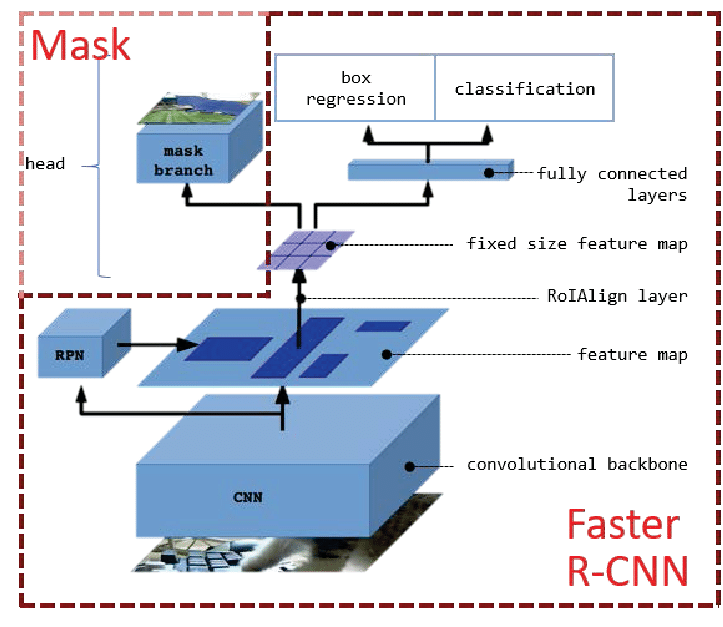
\includegraphics[width=0.69\linewidth]{./image/maskrcnn.png}
  \caption{Mask R-CNN architecture. \textit{Source:~\cite{fig1}, pag. 3.}\\ The convolutional \textit{backbones} (in the lower part of the figure) proposed in the paper are C4, C5 and FPN~\cite{FPN}. For \textit{heads} (in the upper part of the figure) the backbone must include the 5-th stage of ResNet~\cite{Authors5_ResNet}, "res5".}%Le convolutional backbones proposte nel paper sono  C4, C5 e FPN. Per le head la backbone deve includere il 5-th stage of
%ResNet ("res5").}
  \label{fig:mask_rcnn}
\noindent
\end{figure}
\indent BlendMask~\cite{Authors2_BlendMask} is derived from the limits of Mask R-CNN. The authors of the paper define how Mask R-CNN strongly constrains the speed and quality of mask generation at heads, thus making it difficult to deal with complicated scenarios and placing a limit on masks resolution. Furthermore, Mask R-CNN presents itself as an inflexible framework for multi-task networks.They thus attempted to cobine top-down and bottom-up search strategies in FCOS~\cite{fcos}, anchor box-free one-stage approach, which seems able to outperform its two-stage counterparts in terms of accuracy. The architecture of BlendMask, Figure \ref{fig:blendmask}, consists of a detector network and a mask branch. The latter is partitioned in 3 parts: the bottom module that deals with predicting scores maps, called bases; the top layer composed of a single convolution layer and towers, as many as the input features, with the task of predicting attention instances; and a blender module that combines scores with attentions.
%\indent BlendMask~\cite{Authors2_BlendMask} deriva dai limiti di Mask R-CNN~\cite{Authors1_maskrcnn}. Gli autori del paper definiscono come Mask R-CNN~\cite{Authors1_maskrcnn} vincoli fortemente la velocit\`a e la qualit\`a di generazione delle maschere alle heads, facendo cos\`i fatica a trattare scenari complicati e ponendo un limite alla risoluzione delle maschere. Inoltre Mask R-CNN~\cite{Authors1_maskrcnn} si presenta come un framework poco flessibile per reti multi-task. Hanno cos\`i cercato di cobinare strategie di ricerca dall'alto verso il basso e dal basso verso l'alto in FCOS~\cite{fcos}, one stage approch, che sembra in grado di superare le controparti a due stadi in termini di precisione. L'architettura di BlendMask~\cite{Authors2_BlendMask}, Figure \ref{fig:blendmask}, si compone di un detector network e di una mask branch. Quest'ultima \`e partizionata in 3 parti: il modulo inferiore che si occupa di prevedere le scores map, chiamate basi; the top layer composto da un singolo strato di convoluzione e da torri, tante quante sono le input features, con il compito di predirre attention instance; e un modulo blender che unisce scores con attenzioni.
\begin{figure}[H]
\centering
  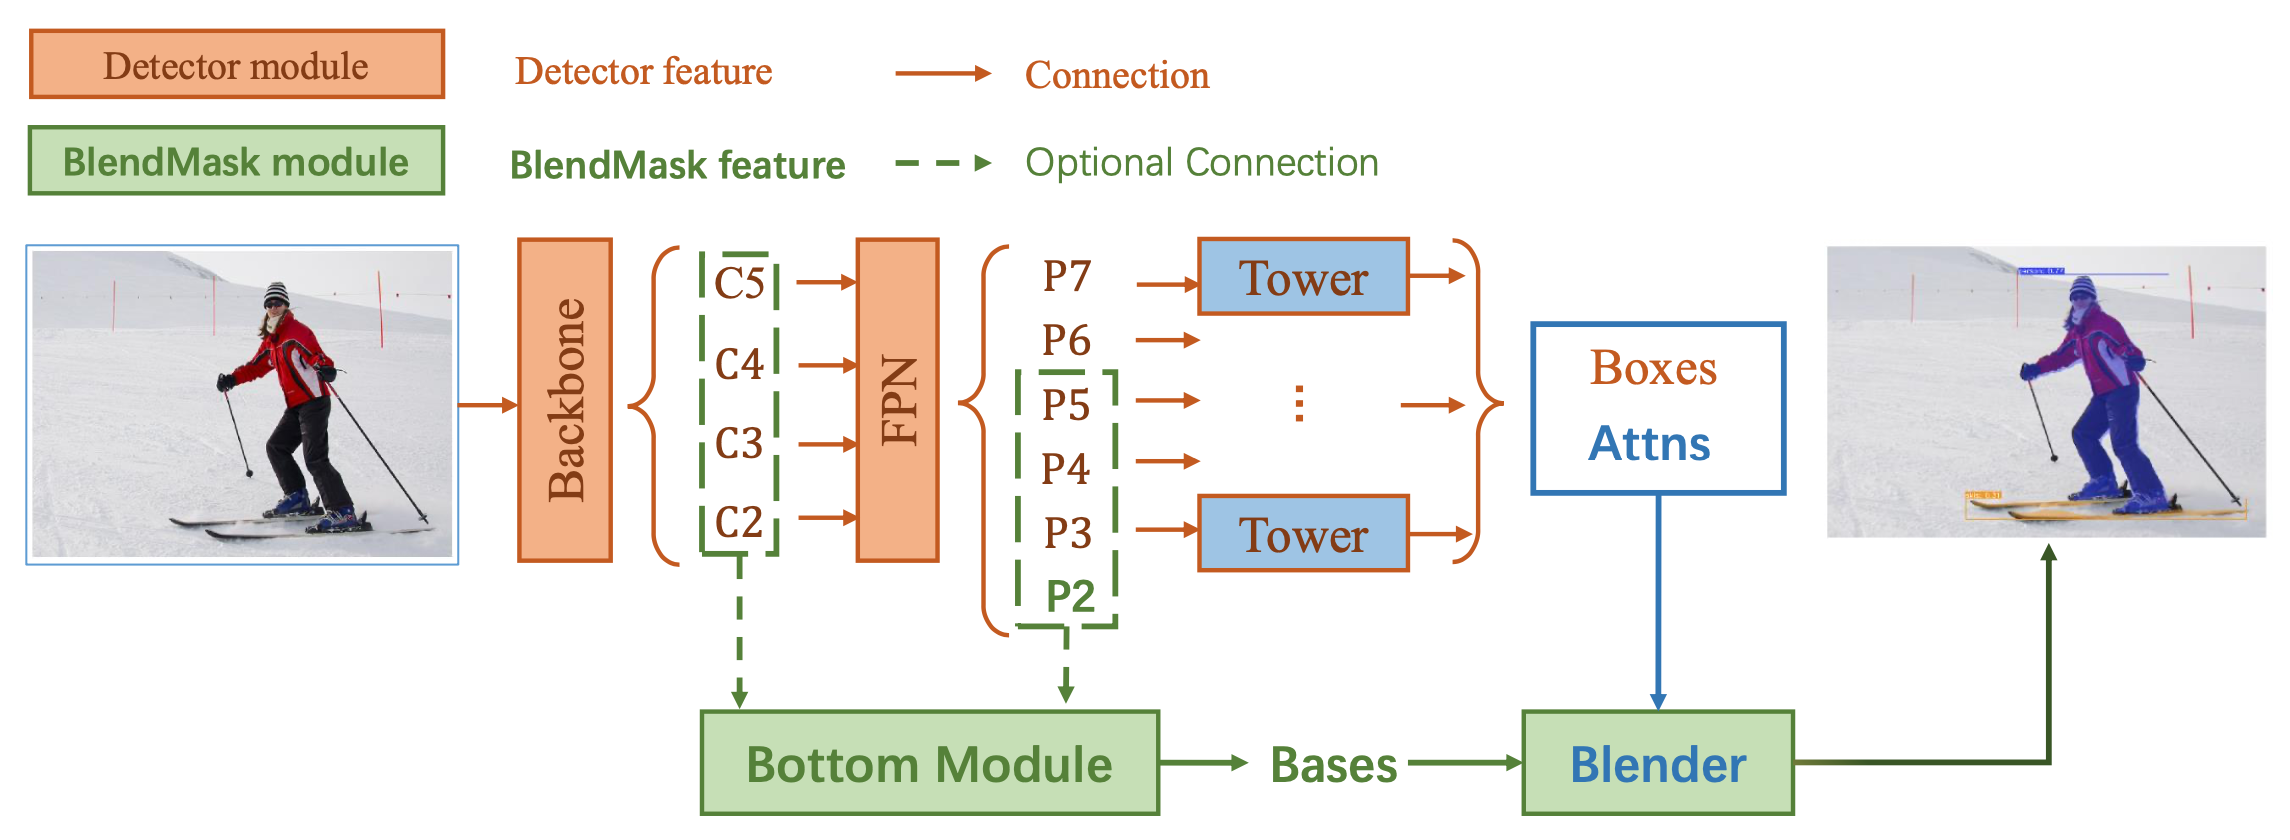
\includegraphics[width=1\linewidth]{./image/blendmask.png}
  \caption{BlendMask architecture. \textit{Source:~\cite{Authors2_BlendMask}, pag. 3.} \\ The \textit{bottom module} (to left) uses C4/C5 or FPN~\cite{FPN} and produces the bases. In the \textit{top layer} (to right) a single convolution layer is added above the towers and this allows attention masks to be produced. The \textit{blender module} (lower part of the figure), for each instance combining bases linearly with the learned attention maps.}
  %Il modulo inferiore (a destra) usa funzionalit\`a backbone o FPN,  a seconda assume funzioni "C" o "P" come input, e produce le basi. Nel modolo superiore (a sinistra) al di sopra delle torri viene aggiunto un singolo strato di convoluzione, e questo permette di produrre maschere di attenzione, insieme a ciascuna previsione del riquadro di delimitazione. Il modulo di blender (parte bassa della figura), per ogni istanza ritaglia le basi con il suo riquadro di delimitazione, combinadole linearmente con le mappe di attenzione apprese.}
  \label{fig:blendmask}
\noindent
\end{figure}
\noindent
\indent SOLOv2~\cite{Authors6_SOLOv2} is box-free one-stage approach, a successor of SOLO~\cite{solo}.
In this case each instance of an image is segmented dynamically, without detection of the bounding box.
The mask generation, unlike Mask R-CNN, is decoupled into mask kernel prediction and mask feature learning. These two elements are responsible for generating convolution kernels and feature maps. SOLOv2 also manages to achieve promising results through the use of the matrix \textit{non-maximum suppression} (NMS) technique, proposed by the authors of the paper, which reduces duplicate predictions while gaining less inference overhead.
%\indent SOLOv2~\cite{Authors6_SOLOv2} \`e un altro approccio a singolo stage, sucessore di SOLO~\cite{solo}. In questo caso ogni istanza di un'immagine viene segmentata dinamicamente, senza rilevamento del riquadro di delimitazione.
%La generazione della maschera, a differenza di Mask R-CNN~\cite{Authors1_maskrcnn}, \`e disaccoppiata in mask kernel prediction e in mask feature learning. Questi due elementi sono responsabili della generazione dei convolution kernels e delle feature maps. SOLOv2~\cite{Authors6_SOLOv2} riesce a ottenere risultati promettenti anche grazie all'uso della matrix non-maximum suppression (NMS) technique, che riduce le previsioni duplicate guadagnandone in minor overhead d'inferenza.
\subsection{Contour-based approach}
Deep Snake~\cite{Authors7_deepsnake} is a contour-based approach, implementing the idea of snake algorithms with a learning-based approach. Deep Snake consists of a two-stage pipeline: in a first instance there is an initial contour proposal on the object of an image; followed by the use of a Neural Network, which iteratively deforms this proposal until it exactly matches the object's boundaries. For learning the structure of contour features, the authors of the paper propose the use of \textit{Circular Convolution}.
%Deep Snake~\cite{Authors7_deepsnake} \`e un approccio basato su contorni, che implementa l'idea degli algoritmi snake con learning-based approach. Deep Snake~\cite{Authors7_deepsnake} si compone di una pipeline a due stadi: in un prima istanza vi \`e  una proposta di controno iniziale sull'oggetto di un'immagine; fatta successivamente seguire dall'uso di una Rete Neurale, che deforma iterativamente questa proposta, fino a farla combacire esattamente con i confini propri dell'oggetto. Per l'apprendimento della struttura delle features del contorno, gli autori del paper propongono l'uso della Circular Convolution.

\section{Datasets}
The datasets of \textit{Urban Street Scenes}, which we used, belong to \textit{Cityscapes}~\cite{cityscapes} and \textit{WildDash}~\cite{wildDash}.
%I datasets di \textit{Urban Street Scenes}, che abbiamo usato, appartengono a \textit{Cityscapes}~\cite{cityscapes} e \textit{WildDash}~\cite{wildDash}.
\subsection{Cityscapes}
\textit{Cityscapes}~\cite{cityscapes} is a suite of benchmark and a large-scale dataset for semantic urban scene understanding. It is suitable for learning and testing pixel-level and instance-level semantic labelling methods.  The images of \textit{Cityscapes} were created from a large and diverse set of video sequences, recorded in 50 different cities. These may be inclusive of high quality annotations, or/and coarse annotations; the latter allow the testing of methods employing large volumes of weakly labelled data. The annotations contained, which are fundamental for the evaluation of a model, are of a polygonal type.
The dataset we used, belonging to \textit{Cityscapes}, is partitioned into two units: \textit{gtFine} and \textit{leftImg8}, which we used in pairs. \textit{gtFine} consists of fine annotations for 3 475 train and val images, and 1 525 test set images.
\textit{leftImg8} from "row" images of urban traffic, with train set, test set and val set; a total of 5 000 images.
%\textit{Cityscapes}~\cite{cityscapes} \`e una suite di benchmark e un dataset su larga scala per semantic urban scene understanding. \`E adatto per apprendere e testare metodi pixel-level e instance-level semantic labeling. Le immagini di \textit{Cityscapes}~\cite{cityscapes} sono state create da un'insieme vasto e diversificato di sequenze video, registrate in 50 citt\`a diverse. Queste possono essere comprensive di annotazioni di alta qualit\`a, o/e di tipo grossolane; quest'ultime consentono di testare metodi che impiegano grandi volumi di dati debolmente etichettati. Le annotazioni contenute, fondamentali per la valutazione di un modello, sono di tipo poligonale.\\ 
%Il dataset che abbiamo usato, appartenete a \textit{Cityscapes}~\cite{cityscapes}, si partiziona in due unit\`a: \textit{gtFine} e \textit{leftImg8} (Figure \ref{fig:image_gtfine}), che abbiamo utilizzato in coppia. \textit{gtFine} si compone di annotazioni fini per 3 475 immagini di train e val, e 1 525 immagini per test set. \textit{leftImg8} da immagini "row" di traffico urbano, con train set, test set e val set; per un totale di 5 000 immagini.
%\begin{figure}[H]
%\centering
%  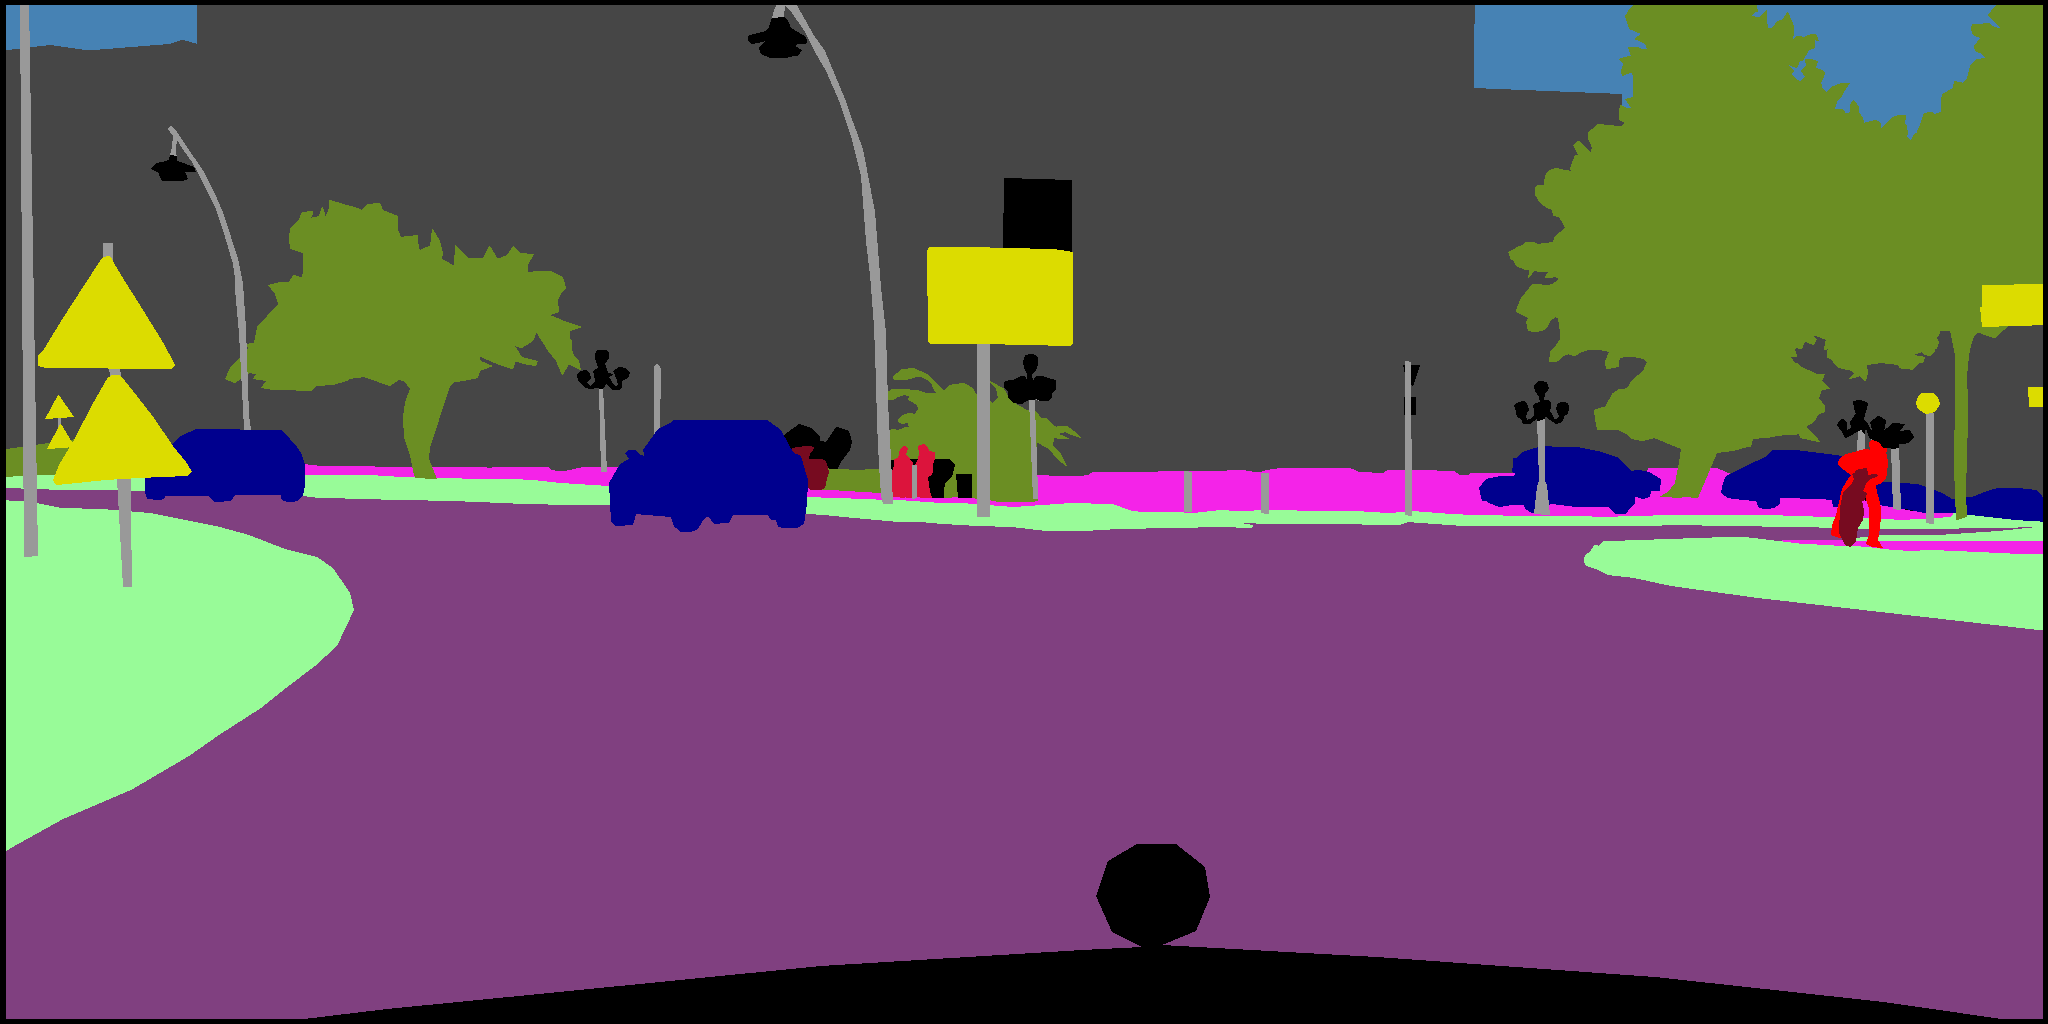
\includegraphics[width=0.41\linewidth]{./image/gtFine.png} \quad 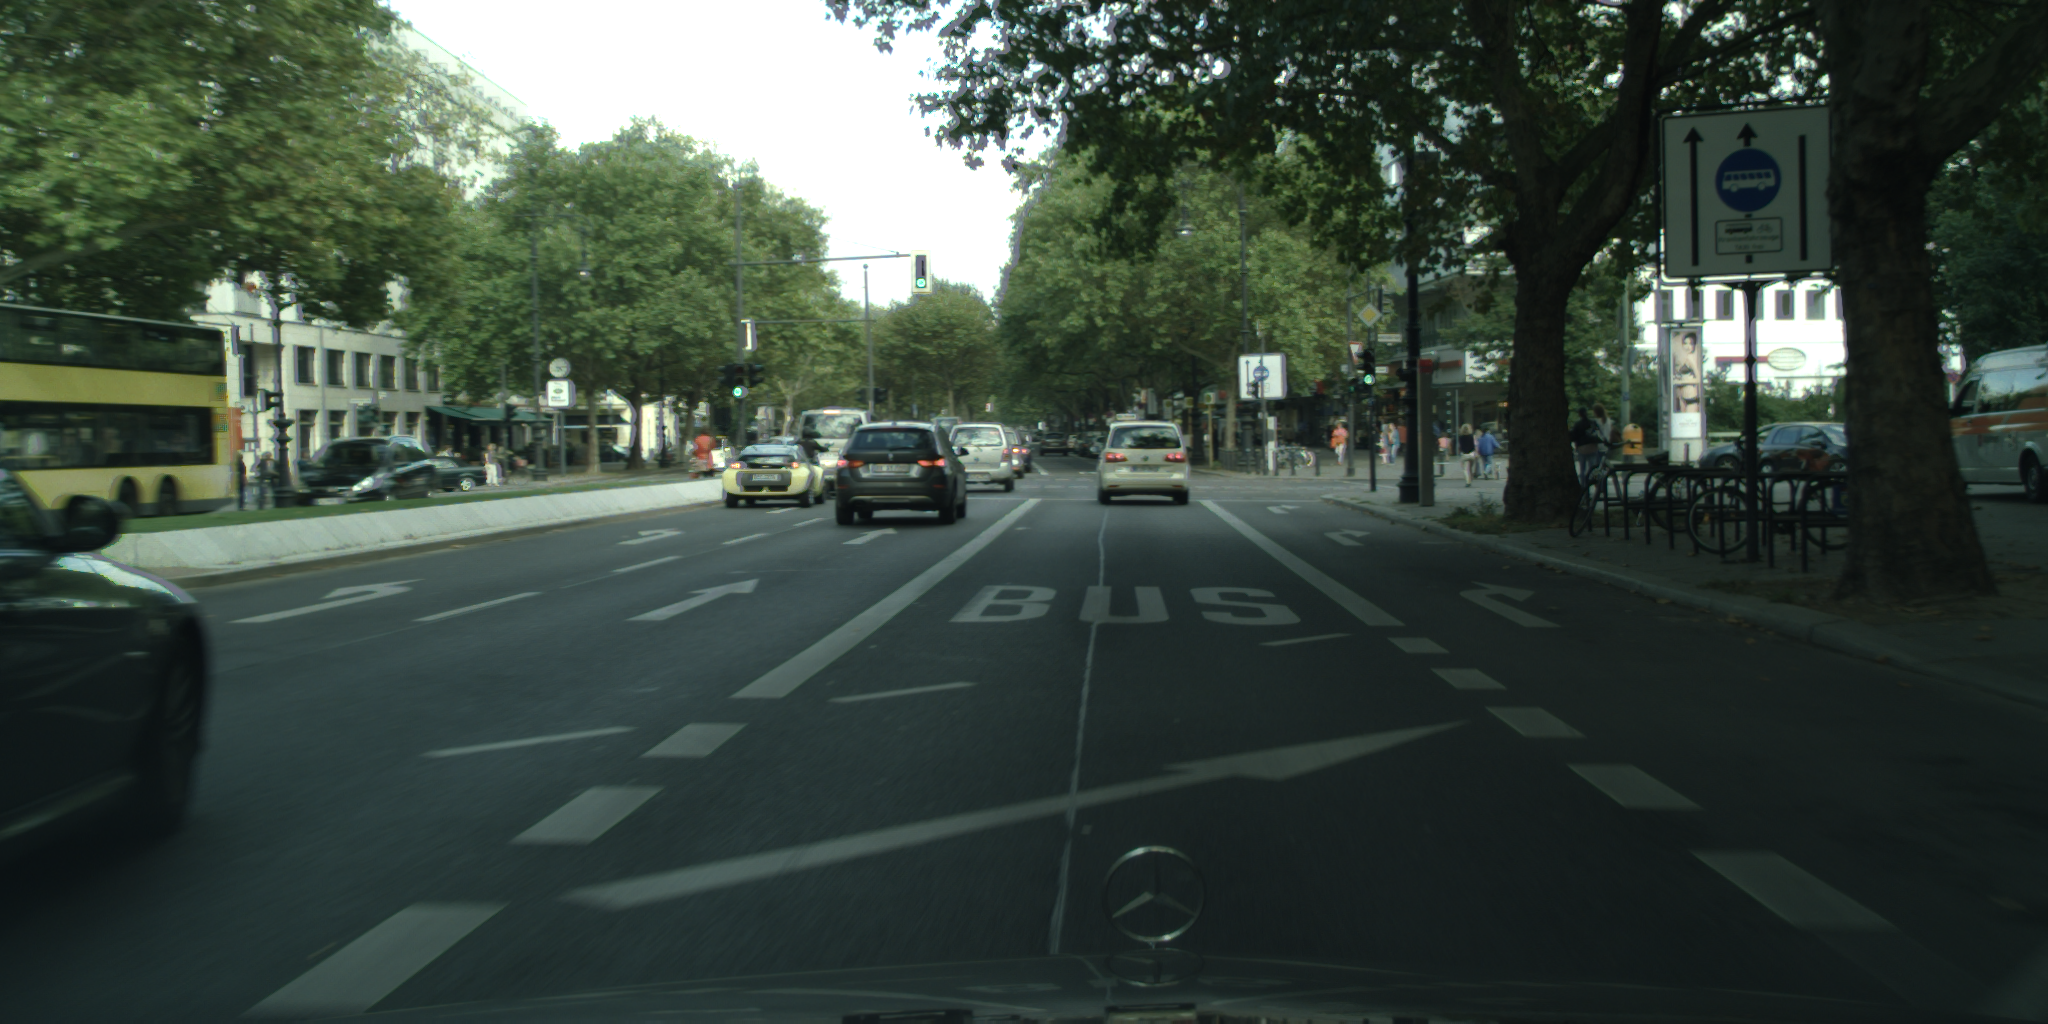
\includegraphics[width=0.41\linewidth]{./image/leftImg8.png}
 % \caption{\textit{Cityscapes}~\cite{cityscapes} images: \textit{gtFine} to left and \textit{leftImg8} to right.}
%  \label{fig:image_gtfine}
%\noindent
%\end{figure}
In Figure \ref{fig:class_definitions_city}, we report the classes and the number of occurrences in \textit{gtFine train} and \textit{leftImg8 train}. The total number of classes is 8.
%In Figura \ref{fig:class_definitions_city}, riportiamo le classi e il numero di occorrenze in \textit{gtFine train} e \textit{leftImg8 train}. Il numero di classi complessive sono 8.
\begin{figure}[H]
\centering
  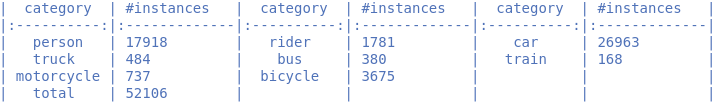
\includegraphics[width=0.9\linewidth]{./image/city_class} 
  \caption{\textit{Cityscapes}: definitions of train dataset classes.} %\\ The class considered "dangerous" for a good generalisation of a model is \textit{train}, due to the small number of instances (168).}
  \label{fig:class_definitions_city}
\noindent
\end{figure}
However of \textit{Cityscapes} although the datasets include several months and seasons, they are always images taken in good weather conditions. This aspect prompted us to analyse the behaviour of our instance segmentation techniques on the \textit{WildDash}~\cite{wildDash} dataset.
%Tuttavia i datasets di \textit{Cityscapes}~\cite{cityscapes} anche se includono diversi mesi e stagioni, sono sempre immagini scattate in buone condizioni metereologiche. Questo aspetto ci ha spinto ad analizzare il comportamento delle nostre tecniche di instance segmentation anche sul dataset \textit{WildDash}~\cite{wildDash}.

\subsection{WildDash}
\label{dataset_wd}
\textit{WildDash}~\cite{wildDash} is a benchmark suite and dataset for semantic and instance segmentation for the automotive domain. The images, contained in the datasets, come from different sources from all over the world. In addition, they present scenarios, such as rain, darkness and road cover, which are real challenges for image recognition. This highlights the shortcomings of any instance segmentation technique.
The dataset we used is \textit{public gt package} consisting of 4 256 images, aimed specifically at solving instance segmentation tasks; however, was not divided into train, val and test set. Consequently, we decided to divide it up manually, reserving 3 405 images as train set and 851 images as test set. We did not consider it necessary to make a further partition in val set, in order to keep as many images as possible in the training; and assuming that our models, using weights already pretrained on \textit{ImageNet}~\cite{imagenet}, were accurate enough not to require \textit{Model Selection}.
%\textit{WildDash}~\cite{wildDash} \`e una suite di benchmark e un dataset per la segmentazione semantica e d'instanza per il dominio automobilistico. Le immagini, contenute nei datasets, provengono da diverse fonti da tutto il mondo. Inoltre presentano scenari, quali pioggia, oscurit\`a, copertura stradale che sono delle vere e proprie challenge per il riconoscimento delle immagini. Questo consente di mettere in luce le carenze di una qualsiasi tecnica di instance segmentation.\\
%Il dataset che abbiamo usato \`e \textit{public gt package} (Figure \ref{fig:image_wd}), composto da 4 256 immagini, rivolto appositamente a risolvere tasks di instance segmentation; non era tuttavia suddiviso in train, val e test set. Abbiamo di conseguenza deciso di suddividerlo manualmente, riservando 3 405 immagini come train set e 851 immagini come test set. Non abbiamo ritenuto necessario fare un'ulteriore partizione in val set, in modo da mantenere pi\`u immagini possibili nel addestramento; e assumendo che i nostri modelli, usando pesi gi\`a preadestrati su ImageNet~\cite{imagenet}, fossero sufficientemente accurati da non richiedere model selection.
%\begin{figure}[H]
%\centering
%  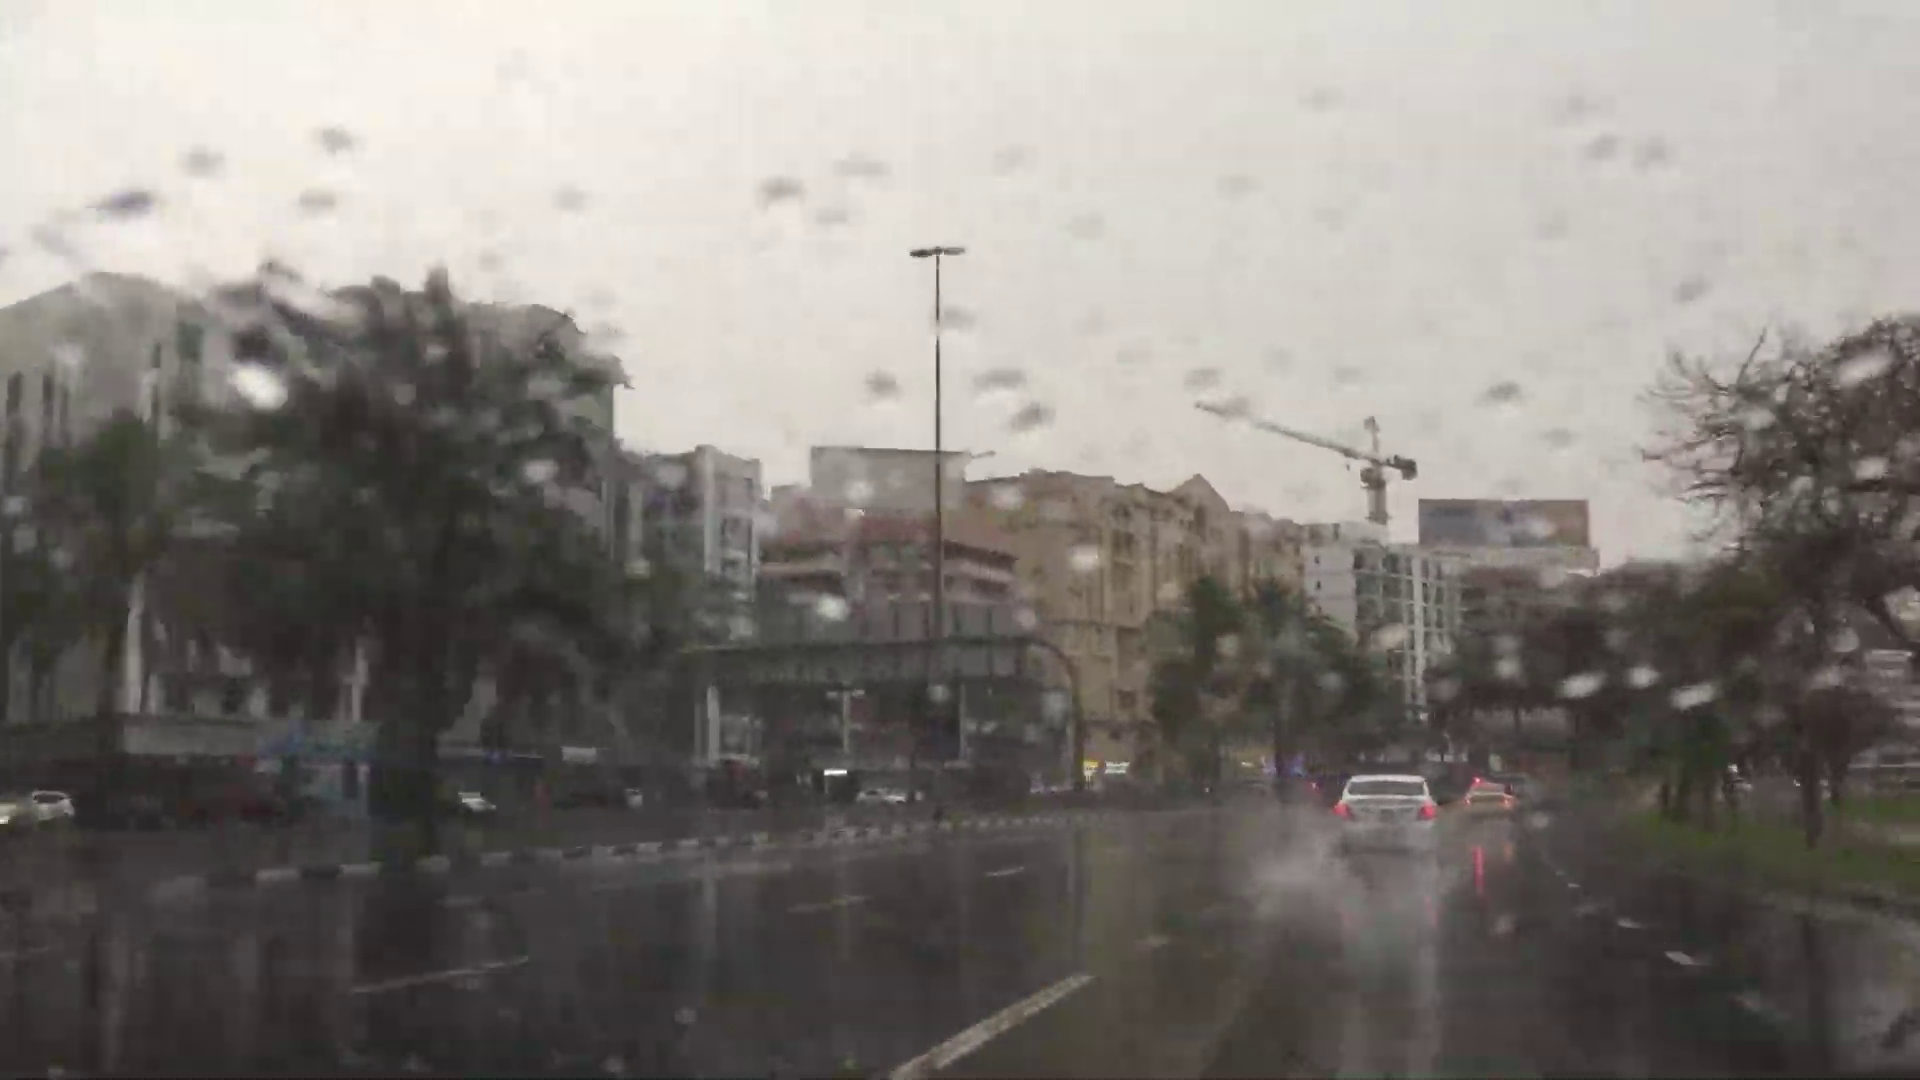
\includegraphics[width=0.4\linewidth]{./image/wd_rain.jpg} \quad 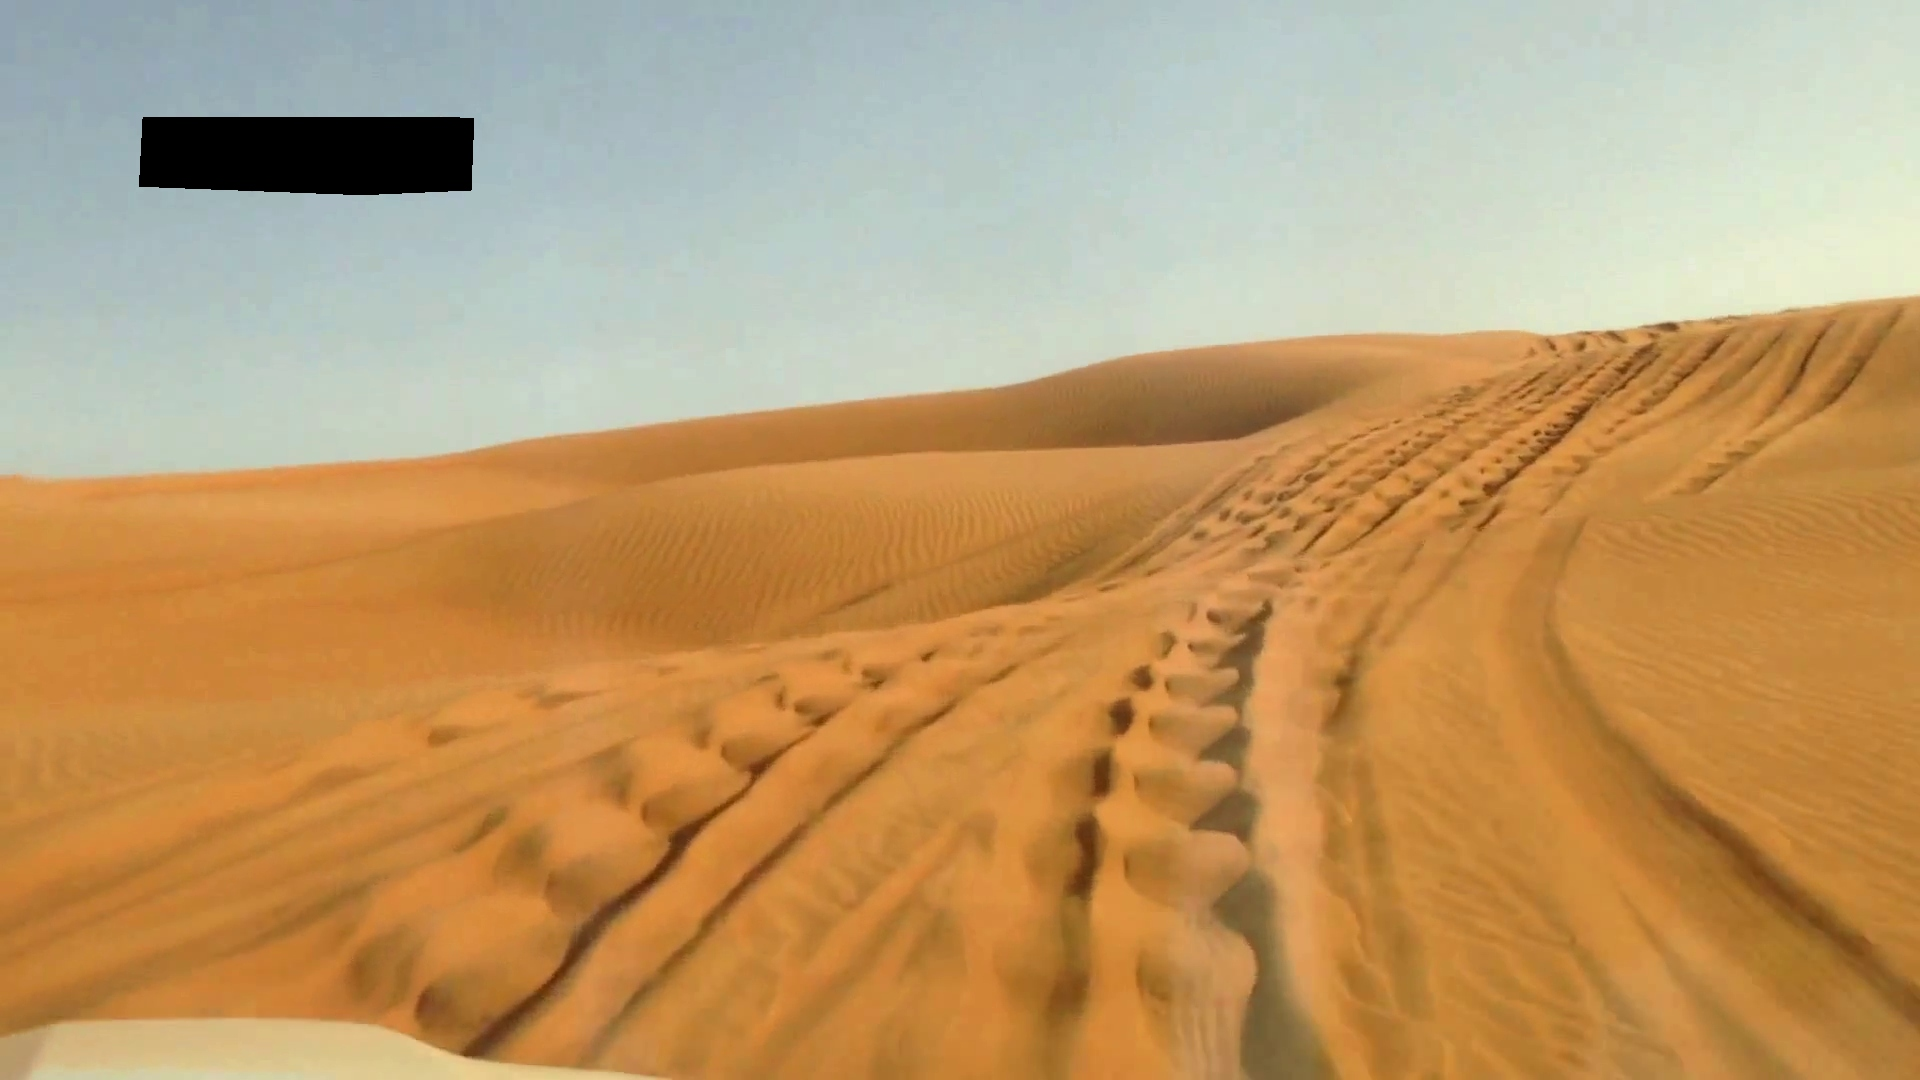
\includegraphics[width=0.4\linewidth]{./image/wd_desert.jpg}
%  \caption{\textit{WildDash}~\cite{wildDash} images:  \textit{rain scenario} to left and \textit{road in the desert} to right.}
%  \label{fig:image_wd}
\noindent
%\end{figure}
In Figure \ref{fig:class_definitions_wd}, we report the classes and the number of occurrences in \textit{public gt package train}. The total number of classes is 13.
%In Figura \ref{fig:class_definitions_wd}, riportiamo le classi e il numero di occorrenze in \textit{public gt package train}. Il numero di classi complessive sono 13.
\begin{figure}[H]
\centering
  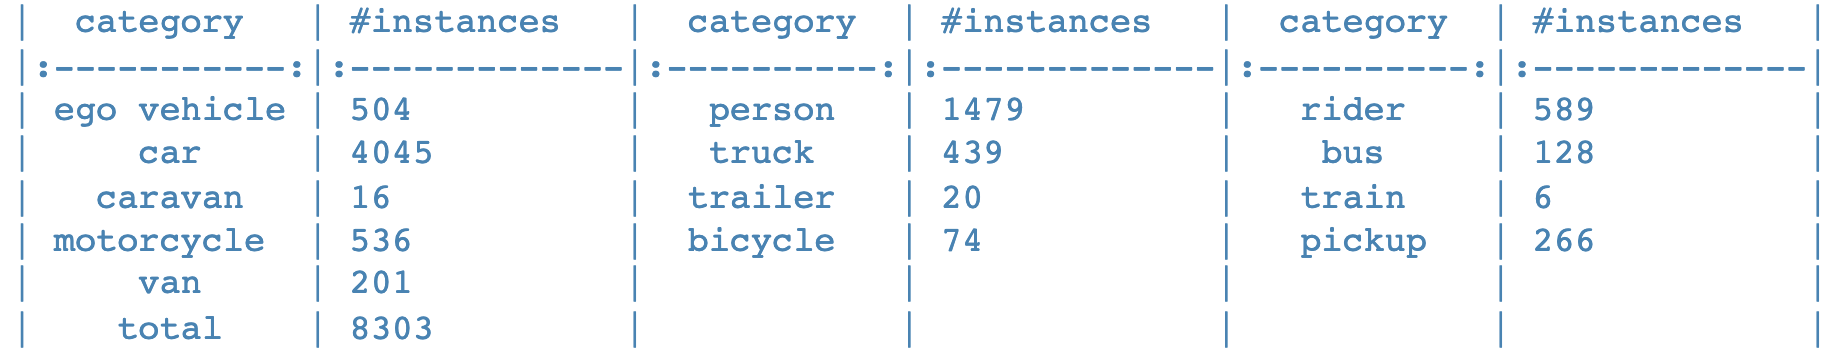
\includegraphics[width=0.9\linewidth]{./image/wd_class.png} 
  \caption{\textit{WildDash}: definitions of train dataset classes.} %\\ The classes considered "dangerous" for a good generalisation of a model are \textit{caravan} (46), \textit{trailer} (65) and \textit{train} (74).}
  \label{fig:class_definitions_wd}
\noindent
\end{figure}


\section{Method}
In order to be able to operationally compare the instance segmentation techniques, that are the subject of our work, we have referred to already existing libraries, developed by the researchers of~\cite{Authors1_maskrcnn, Authors2_BlendMask}.  These are \textit{Detectron2} for Mask R-CNN~\cite{Authors1_maskrcnn} and \textit{AdelaiDet} for BlendMask~\cite{Authors2_BlendMask}.
These libraries have allowed us to define sub-optimal ideal models, in order to improve their accuracy during experiments. Furthermore, making explicit the evaluation set and the metrics needed to estimate performance, allowed us to concretise the concept of comparison.
%Per poter operativamente confrontare le tecniche di instance segmentation oggetto del nostro lavoro, abbiamo fatto riferimento a librerie gi\`a esistenti, sviluppate dai ricercatori di ~\cite{Authors1_maskrcnn} e \cite{Authors2_BlendMask}. Queste sono \textit{Detectron2} per Mask R-CNN~\cite{Authors1_maskrcnn} e \textit{AdelaiDet} per BlendMask~\cite{Authors2_BlendMask}.
%Tali librerie ci hanno consentito di definire modelli ideali subottimi, con il fine di migliorarne la precisione durante gli esperimenti. Inoltre anche esplicitare il set valutazione e le metriche necessarie per stima di performance, ci hanno consentito di concretizzare il concetto di confronto.

\subsection{Architecture}
We decided to use ResNet-101-FPN as the backbone in both Mask R-CNN~\cite{Authors1_maskrcnn} and BlendMask~\cite{Authors2_BlendMask}. In addition, as the bottom module of BlendMask we have instantiated ProtoNet~\cite{protonet}. 
%Abbiamo deciso di utilizzare ResNet-101-FPN come backbone sia in Mask R-CNN~\cite{Authors1_maskrcnn} che in BlendMask~\cite{Authors2_BlendMask}. Inoltre come bottom module di BlendMask~\cite{Authors2_BlendMask} abbiamo istanziato ProtoNet~\cite{protonet}. 
\subsubsection{ResNet 101}
Both \textit{Detectron2} and \textit{AdelaiDet} offer ResNet~\cite{Authors5_ResNet} as a backbone network, in which it is possible to choose between 50 and 101 layers.  In addition, \textit{Detectron2} also includes ResNeXt~\cite{resxt} 101, a cardinal variant of ResNet 101; which, however, we have excluded from any possible comparison because of the excessive training time, for the means at our disposal.
We considered ResNet 101, Figure \ref{fig:resnet101}, sufficient for our purposes, defined as a network that also converges very well from the reference paper~\cite{Authors5_ResNet}.
%Sia \textit{Detectron2} che \textit{AdelaiDet} offrono come rete backbone ResNet~\cite{Authors5_ResNet}, in cui \`e possibile scegliere tra 50 e 101 layers. Inoltre \textit{Detectron2} include anche ResNeXt~\cite{resxt} 101, variante con cardinalit\`a di ResNet 101; che tuttavia abbiamo escluso da ogni possibile confronto a causa dell' eccessivo tempo di training, per i mezzi  a nostra disposizione, non giustificabile dal solo aumento di accuracy della maschera.
%Abbiamo ritenuto ResNet 101, Figure \ref{fig:resnet101} sufficiente ai nostri scopi, definita come una rete che converge molto bene anche dal paper di riferimento~\cite{Authors5_ResNet}.
\begin{figure}[H]
\centering
  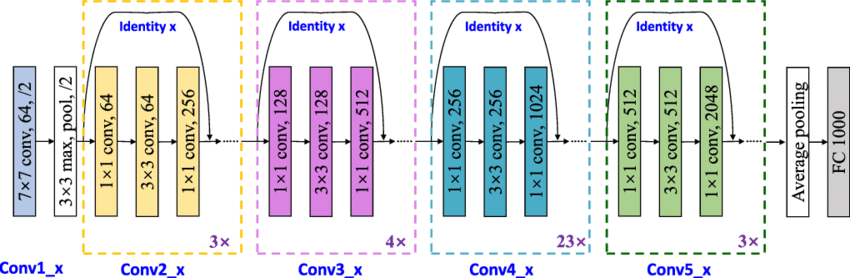
\includegraphics[width=0.90\linewidth]{./image/resnet101.png} 
  \caption{The structure of the ResNet 101. \textit{Source: ~\cite{resnet101_img}, pag. 6.}\\
  The figure shows Resnet 101. It uses skip connections, i.e. arcs over each block, to solve the problems associated with gradient computation.}%In figura viene prsentata Resnet 101, una Residual Neural Network (CNN$+$deepness) with 101 layers. Essa usa le skip connections, ovvero gli archi sopra ciascun blocco, per risolvere i prolemi legati alla computazione del gradiente.}
  \label{fig:resnet101}
\noindent
\end{figure}
\subsubsection{Feature Pyramid Network}
For complete the backbone, ResNet~\cite{Authors5_ResNet} it is not enough. Is necessary a second architecture that extract the features in Mask R-CNN~\cite{Authors1_maskrcnn} or the basis for BlendMask~\cite{Authors2_BlendMask}. In this case \textit{Detectron2} includes several already configured approaches, e.g. C4 where features are extracted from the 4-th convolutional stage of ResNet; or FPN~\cite{FPN} with lateral connections that allow to build a pyramid of functionalities within the network from single-scale input. \textit{AdelaiDet}, on the other hand, exclusively implements FPN. Our choice fell on FPN, in order to maintain consistency between the two models under analysis, and to be once again in line with what was defined by the papers~\cite{Authors1_maskrcnn, Authors2_BlendMask}.  In fact, the researchers declare as FPN is performant in both features/bases extraction and execution time.  In Figure \ref{fig:FPN} we show how FPN solves the feature extraction, when it is used as backbone in an instance segmentation task.
%Per completare la backbone ResNet~\cite{Authors5_ResNet} non basta, \`e necessaria anche una seconda architettura che si occupi di estrarre le caratteristiche in Mask R-CNN~\cite{Authors1_maskrcnn} o le basi per BlendMask~\cite{Authors2_BlendMask}. In questo caso \textit{Detectron2} include diversi approcci gi\`a configurati, ad esempio C4 dove vengono estratte le caratteristiche dal quarto stadio convoluzionale di ResNet~\cite{Authors5_ResNet}; o FPN~\cite{FPN} con connessioni laterali che consentono di costruire una piramide di funzionalit\`a all'interno della rete from single-scale input. \textit{AdelaiDet}, di contro, vede implementato esclusivamente FPN~\cite{FPN}. La nostra scelta \`e ricaduta su FPN~\cite{FPN}, in modo da mantenere coerenza tra i due modelli in analisi, e essere ancora una volta in linea con quanto definito dai papers~\cite{Authors1_maskrcnn},~\cite{Authors2_BlendMask}. I riceratori difatti dichiarano FPN~\cite{FPN} performante  sia per l'estrazione delle features/basi che nel tempo di esecuzione. In Figure \ref{fig:FPN} mostriamo come FPN~\cite{FPN} risolve il compito di estrazione delle features, quando viene utilizzata come backbone in un task di instance segmentation.
\begin{figure}[H]
\centering
  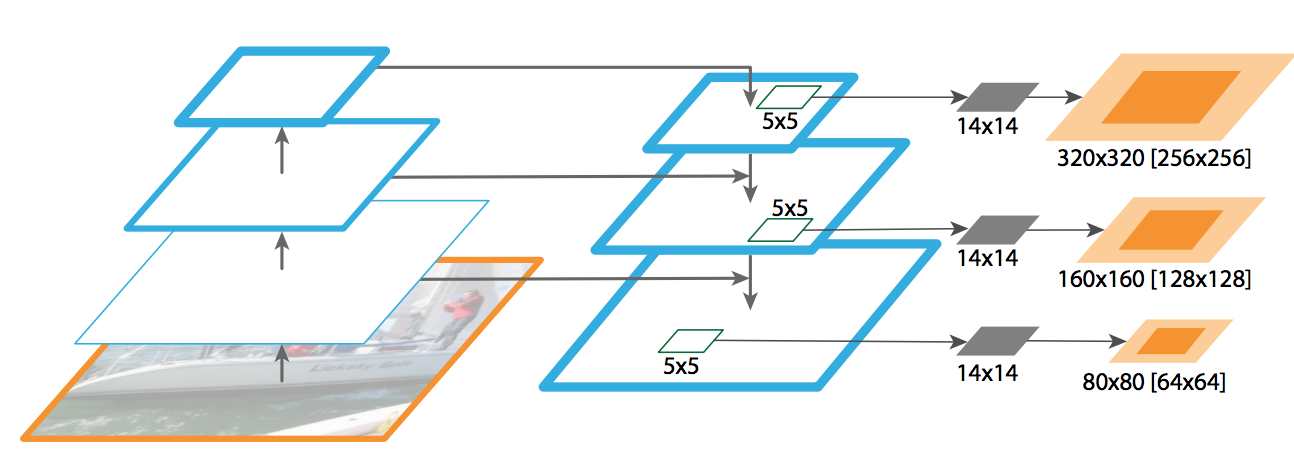
\includegraphics[width=0.8\linewidth]{./image/FPN.png} 
  \caption{FPN for object segment proposals. \textit{Source:~\cite{FPN}, pag. 8.}\\
  The feature pyramid is constructed with identical structure as for object detection.  Each level of the pyramid tries to detect all instances present in an image. A features map/bases is produced for each of these layers, and each will produce a mask. These latter will be combined into a single final mask.}%Ogni livello della piramide cerca di rilevare tutte le istanze presenti in un'immagine. Per ognuno di questi livelli viene prodotta una features map/basi, e ciascuna produrr\`a una maschera. Quest'ultime verranno combinate in un unica maschera finale.}
  \label{fig:FPN}
\noindent
\end{figure}


\subsubsection{ProtoNet decoder}
In \textit{AdelaiDet} there are two types of bottom modules, which receive input from the backbone: ProtoNet~\cite{protonet} and DeepLabv3$+$~\cite{deeplab}. ProtoNet is a prototype generation branch, i.e. it predicts a set of k prototypes masks for the whole image. It is implemented as a Fully Connected Network, where the last layer of which has as many channels as there are prototypes. DeepLabv3$+$ is an encoder-decoder structure, that is able to control the resolution of feature extracts thanks to the \textit{atrous convolution}, which has the effect of increasing the kernel's field of view. In the default configuration of \textit{AdelaiDet}, ProtoNet is defined as a module. We have decided to remain in line with this choice for our sub-optimal model.
% The latter should bring advantages in the balance between accuracy and execution time of the decoder.
%In \textit{AdelaiDet} sono presenti due tipologie di bottom module, che ricevono in input la backbone: ProtoNet~\cite{protonet} and DeepLabv3$+$~\cite{deeplab}. ProtoNet~\cite{protonet} \`e un ramo di generazione di prototipi, ovvero predice un insieme di k maschere prototipo per l'intera immagine. Viene implementata come Fully Connected Network, il cui ultimo strato ha tanti canali quanti sono i prototipi. DeepLabv3$+$~\cite{deeplab} \`e una encoder-decoder structure, che  i\`e in grado di controllare la risoluzione delle features extract grazie alla \textit{atrous convolution}, che ha l'effetto di aumentare il campo visivo del kernel. Quest'ultimo aspetto dovrebbe portare vantaggi nel bilanciamento tra precisione e tempo di esecuzione del decoder.
%Nelle configurazioni di default di AdelaiDet \`e definito ProtoNet come modulo. Abbiamo deciso di rimanere anche noi, per il nostro modello subottimo, in linea con tale scelta.


\subsection{Configuration hyperparameters}
Hyperparameters of configurationHyperparameters of configurationHyperparameters of configurationHyperparameters of configurationHyperparameters of configurationHyperparameters of configurationHyperparameters of configurationHyperparameters of configurationHyperparameters of configurationHyperparameters of configurationHyperparameters of configurationHyperparameters of configurationHyperparameters of configurationHyperparameters of configurationHyperparameters of configurationHyperparameters of configurationHyperparameters of configurationHyperparameters of configurationHyperparameters of configurationHyperparameters of configurationHyperparameters of configurationHyperparameters of configurationHyperparameters of configurationHyperparameters of configurationHyperparameters of configurationHyperparameters of configurationHyperparameters of configurationHyperparameters of configurationHyperparameters of configurationHyperparameters of configuration
\subsection{Loss function}
The loss we used during the training of Mask R-CNN, defined in \cite{Authors1_maskrcnn}, is as follows:
%La loss che abbiamo utilizzato durante il training di Mask R-CNN, definita in \cite{Authors1_maskrcnn}, \`e la seguente:
\begin{equation}
L = L_{cls} + L_{box} + L_{mask} 
\label{loss_mask}
\end{equation}
where:
\begin{itemize}
\item L$_{cls}$ is the classification loss;
\item L$_{box}$ is the bounding-box loss;
\item  L$_{mask}$ is the average binary cross-entropy loss.
\end{itemize}
\noindent
With regard to \textit{BlendMask}, we decided to refer to the semantic loss~\cite{Authors8_semanticloss}, as also done in part of the experiments in~\cite{Authors2_BlendMask}:
%Per quanto riguarda \textit{BlendMask}, abbiamo deciso di fare riferimento alla \textit{semantic loss}~\cite{Authors8_semanticloss}, come fatto anche in parte degli esperimenti in~\cite{Authors2_BlendMask}: 
\begin{equation}
L^s(\alpha, p) \propto - log \sum_{x \models \alpha} \prod_{i:x \models X_i} p_i \prod_{i:x \models \neg X_i} (1-p_i)
\label{Loss_semantic}
\end{equation}
where:
\begin{itemize}
\item $\alpha$ is a sentence in propositional logic, defined on variables $X_1,..X_n$;
%\item $\alpha$ \`e una sentenza in logica proposizionale, definita su variabili $X_1,..X_n$;
\item p is a probability vector for each variable $X_i$;
%\item p \`e un vettore di probabilit\`a per ciascuna variabile $X_i$;
\item $L^s(\alpha, p)$ is the semantic loss between $\alpha$ and p.
%\item $L^s(\alpha, p)$ \`e la perdita semantica tra $\alpha$ e p.
\end{itemize}
\noindent
Intuitively, the semantic loss is proportional to the logarithm of generating a state that satisfies the constraint, when values according to p are sampled. This loss function captures how close the Neural Network is to satisfying the constraints on its output. We decided to add the semantic loss to the loss defined in \ref{loss_mask}, driven by the promising results of the paper~\cite{Authors2_BlendMask} and because it was defined by its authors as useful to achieve state-of-the-art results on semi-supervised multi-class classification. \\
The objective we tried to pursue, both during the definition of the ideal models and during the experiments, was the identification of a trade-off between the minimisation of the loss function, the training time and the accuracy box/mask.
%Intuitivamente  la perdita semantica  \`e proporzionale al logaritmo di generare uno stato che soddisfi il vincolo, quando vengono campionati i valori secondo p. Questa funzione di perdita cattura quanto è vicina la rete neurale al soddisfacimento dei vincoli sul suo output. Abbiamo deciso di aggiungere la \textit{semantic loss} alla loss definita in \ref{loss_mask},  spinti dai risultati prommententi del paper~\cite{Authors2_BlendMask} e perch\`e definita dai suoi stessi autori, come utile per raggiungere risultati all'avanguardia sulla classificazione multi-classe semi-supervisionata. \\
%L'obiettivo che abbiamo cercato di perseguire sia durante la definizione dei modelli ideali che durante gli esperimenti \`e stato l'individuazione di un trade-off tra la minimizzazione della funzione di loss, il tempo di training e AP box/mask.
\subsection{Evalutation}
As far as the evaluation is concerned, we had to settle for the val test dataset of \textit{Cityscapes}. 
This is because one of the choices made by the creators of \textit{Cityscapes}~\cite{cityscapes} not to make the annotations for the test set public, and this makes it impossible to perform any calculations and evaluation on masks and boxes. Instead, as already reported in the section  \S\ref{dataset_wd}, for the \textit{WildDash} dataset, we used the test set, which we partitioned from the train set at 80\%-20\%.
%Per quanto riguarda la valutazione abbiamo dovuto accontentarci per  il dataset di \textit{Cityscapes} del val test. Questo perch\`e una delle scelte degli ideatori di \textit{Cityscapes} \`e di non rendere pubbliche le annotazioni per il test set, e questo fa si che non sia possibile svolgere alcun calcolo di precisione su maschere e box. Invece, come gi\`a riportato nella sezione \S\ref{dataset_wd} per il dataset di \textit{WildDash} abbiamo fatto ricorso al test set, da noi partizionato dal train set risettivamente in quota 80\% - 20\%.

\subsubsection{Metrics}
As a metric for evaluating the results obtained from our models, we decided to use \textit{Average Precision} (AP). The AP calculates the average accuracy value for the recall value from 0 to 1. In formula means:
%Come metrica per la valutazione dei risultati ottenuti dai nostri modelli abbiamo deciso di utilizzare l'Average Precision (AP).
%L'AP  calcola il valore di precisione medio per il valore di richiamo da 0 a 1. In formula significa:
\begin{equation}
\int_0^1 p(r) dr 
\label{AP}
\end{equation}
\noindent
where p(r) is the area under the curve of maximum intersection between \textit{Precision} and \textit{Recall}:
%where p(r) \`e l'area sotto la curva di intersezione massima tra \textit{Precision} and \textit{Recall}:
\begin{itemize}
\item \textit{Recall} measures "how well" all positives are found
\begin{equation}
\frac{\text{true positive}}{\text{true positive + false negative}}
\end{equation}
%\item \textit{Recall} misura "quanto bene" vengono trovati tutti gli positivi, $\frac{\text{true positive}}{\text{true positive + false negative}}$;
\item \textit{Precision} measures the accuracy of predictions
\begin{equation}
\frac{\text{true positive}}{\text{true positive + false positive}}
\end{equation}
%\item Precision l'accuratezza delle previsioni, $\frac{\text{true positive}}{\text{true positive + false positive}}$.
\end{itemize}
\noindent
For our evaluations we decided to consider the AP as is defined metric by COCO, i.e. the AP is averaged over several Intersection over Union (IoU) values.  Specifically, 10 IoU thresholds from the range .50:.05:.95 are used; and from these are extracted the 100 detections with the highest score.
%Per le nostre valutazioni abbiamo deciso di considerare l'AP cos\`i come definita metrica da COCO, ovvero l'AP viene mediata su più valori di Intersection over Union (IoU). Nello specifico vengono utilizzate 10 soglie IoU dall'intervallo .50:.05:.95; e da questi vengono estratti i 100 rilevamenti con il punteggio pi\`u alto.



\subsection{Sub-optimal ideal models results}
\begin{figure}[H]
\centering
 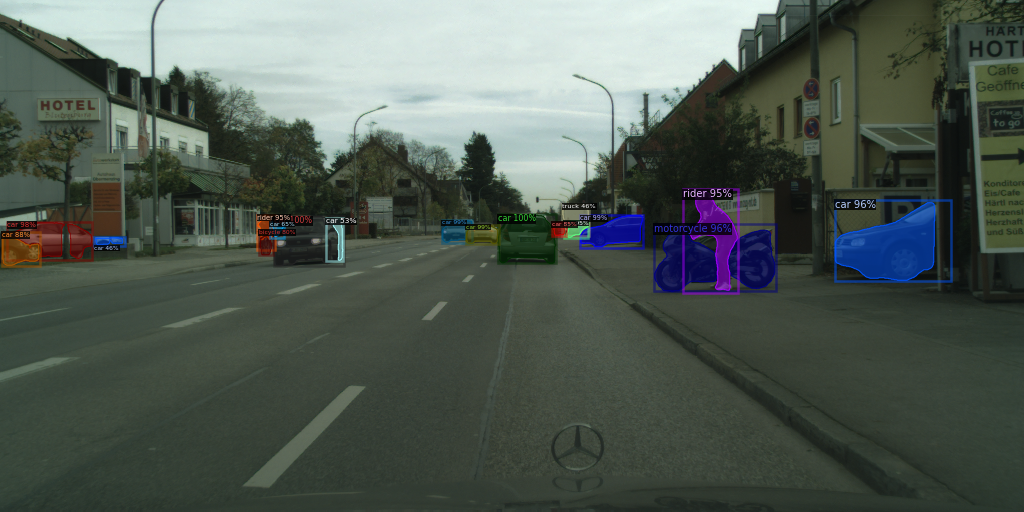
\includegraphics[width=0.45\linewidth]{./image/ideal_model_mask_city.png} 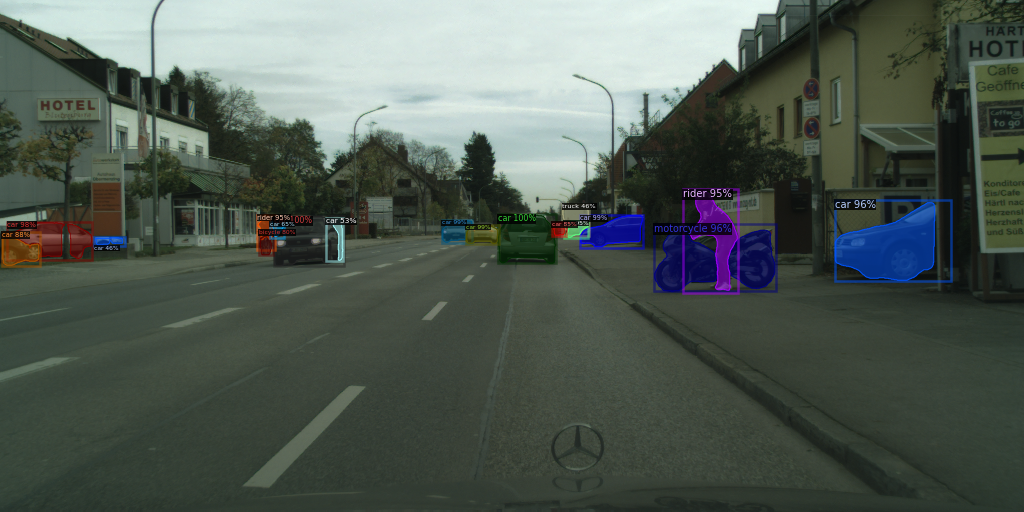
\includegraphics[width=0.45\linewidth]{./image/ideal_model_mask_city.png} 
   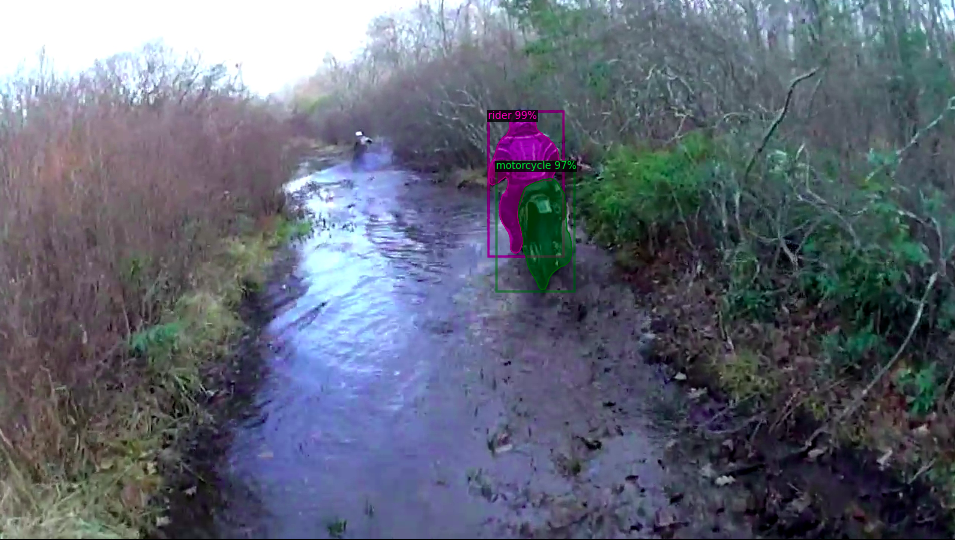
\includegraphics[width=0.45\linewidth]{./image/ideal_model_mask_wd.png}  	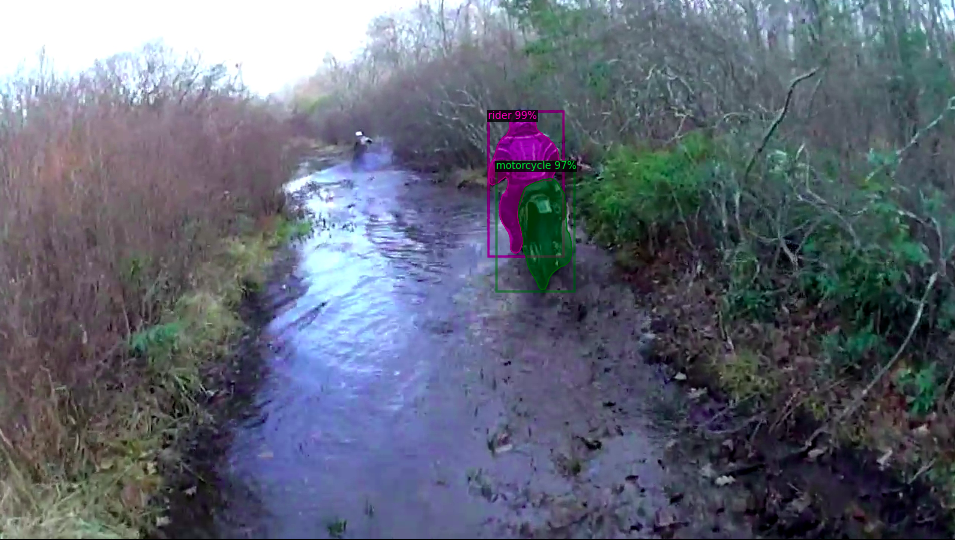
\includegraphics[width=0.45\linewidth]{./image/ideal_model_mask_wd.png}   
  \caption{\textit{Models ideal results}: mask image (to left) and blend image (to right). First row is \textit{Cityscapes} dataset and second row is \textit{WildDash} dataset.}
  \label{fig:result_model_ideal}
\noindent
\end{figure}

\begin{table}[H]
\scriptsize
\begin{center}
\begin{tabular}{|c|c|c|}
\hline
Method & \textit{Cityscapes} & \textit{WildDash}\\
\hline\hline
Mask R-CNN & \begin{tabular}[c]{ccc}box AP: 28.278 \\ mask AP: 23.793 \\ training time:0:26:43\end{tabular} & \begin{tabular}[c]{ccc}box AP: 18.815 \\ mask AP: 17.738 \\ training time: 1:14:57\end{tabular} \\
\hline
BlendMask & &\\
\hline
\end{tabular}
\end{center}
\caption{AP and training time ideal models.}
\label{mytable_deepness_BlendMask}
\end{table}


\section{Experiments}

In questa sezione descriviamo gli esperimenti che abbiamo eseguito per testare  e valutare le tecniche oggetto di questo lavoro. Tali esperimenti gli abbiamo eseguiti al termine delle fasi di studio e codifica.

\subsection{Backbone}
\label{experiments:second_trial}
La seconda serie di esperimenti, che abbiamo compiuto, riguarda la definizione della backbone. Tutte le tecniche a stadi, oggetto del confronto, sono dotate del suddetto modulo inferiore, per cui ci \`e risultato semplice uniformare le scelte architetturali in modo da poter compiere una valutazione oggettiva. Le tecniche che abbiamo confrontato sono state Mask R-CNN e BlendMask.\\
Le configurazioni constanti delle reti sono image size ...,  numero massimo di iterazioni, learning rate ..., step size a ... e fine-tuning esclusivamente agli ultimi 2 livelli.

\begin{table}[H]
\scriptsize
\begin{center}
\begin{tabular}{|c|c|c|}
\hline
Method and architecture & \textit{Cityscapes} AP & \textit{WildDash} AP\\
\hline\hline
\begin{tabular}[c]{cc}Mask R-CNN $+$ ResNet50 \\ $+$ C4 $+$ Base-RCNN-C4\end{tabular} & & \\
\hline
\begin{tabular}[c]{cc}Mask R-CNN $+$ ResNet50 \\ $+$ DC5 $+$ Base-RCNN-DilatedC5\end{tabular} & & \\
\hline
\begin{tabular}[c]{cc}Mask R-CNN $+$ ResNet50 \\ $+$ FPN $+$ Base-RCNN-FPN\end{tabular} & &\\
\hline
\end{tabular}
\end{center}
\caption{Backbone Mask R-CNN result.}
\label{mytable_backbone_MaskRCNN}
\end{table}
\noindent
Per BlendMask, oltre a settare le configurazioni costanti, avvalendoci dei risultati presentati in ... abbiamo settato R $=$ 56, M $=$ 14, K $=$ 4, sampling method for bottom bases bilinear pooling, interpolation method for top-level attentions bilinear upsampling and semantic loss. Inoltre abbiamo deciso di testare vari tipi di decoder: ProtoNet and DeepLabv3+.
\begin{table}[H]
\scriptsize
\begin{center}
\begin{tabular}{|c|c|c|}
\hline
Method and architecture & \textit{Cityscapes} AP & \textit{WildDash} AP\\
\hline\hline
\begin{tabular}[c]{cc}BlendMask with decoder ProtoNet \\ $+$ ResNet50 $+$ FPN $+$ Base-550\end{tabular} & &\\
\hline
\begin{tabular}[c]{ccc}BlendMask with decoder ProtoNet \\ $+$ ResNet50 $+$ deformable convolution \\ $+$ FPN $+$ Base-550\end{tabular} & &\\
\hline
\begin{tabular}[c]{cc}BlendMask with decoder DeepLabv3+ \\ $+$ ResNet50 $+$ FPN $+$ Base-550\end{tabular} & &\\
\hline
\begin{tabular}[c]{ccc}BlendMask with decoder DeepLabv3+ \\ $+$ ResNet50 $+$ deformable convolution \\ $+$ FPN  $+$ Base-550\end{tabular} & &\\
\hline
\end{tabular}
\end{center}
\caption{Backbone BlendMask result.}
\label{mytable_backbone_BlendMask}
\end{table}

\subsection{Deepness}
Una terza serie di esperimenti ha riguardato lo studio della profondit\`a delle reti ResNet.\\
I parametri di configurazione non definiti in modo esplicito, sono le medesime di quelle riportate nella sezione \S\ref{experiments:second_trial}.
\begin{table}[H]
\scriptsize
\begin{center}
\begin{tabular}{|c|c|c|}
\hline
Method and architecture & \textit{Cityscapes} AP & \textit{WildDash} AP\\
\hline\hline
\begin{tabular}[c]{cc}BlendMask with decoder ProtoNet \\ $+$ ResNet101 $+$ FPN $+$ Base-BlendMask\end{tabular} & &\\
\hline
\begin{tabular}[c]{ccc}BlendMask with decoder ProtoNet \\ $+$ ResNet101 $+$ deformable convolution \\$+$ FPN $+$ Base-BlendMask\end{tabular} & &\\
\hline
\end{tabular}
\end{center}
\caption{Deepness BlendMask result.}
\label{mytable_deepness_BlendMask}
\end{table}

\subsection{Freeze levels}
Per la quarta serie di esperimenti ci siamo voluti concentrare sul numero di layers da "scongelare" di ResNet durante il re-training dei pesi.\\
I parametri di configurazione non definiti in modo esplicito, sono le medesime di quelle riportate nella sezione \S \ref{experiments:second_trial}.
\begin{table}[H]
\scriptsize
\begin{center}
\begin{tabular}{|c|c|c|}
\hline
Method and architecture & \textit{Cityscapes} AP & \textit{WildDash} AP\\
\hline\hline
\begin{tabular}[c]{ccc}Mask R-CNN $+$ ResNet101 $+$ FPN \\ 1 layers freeze\end{tabular} & &\\
\hline
\begin{tabular}[c]{ccc}Mask R-CNN $+$ ResNet101 $+$ FPN \\ 3 layers freeze\end{tabular} & &\\
\hline
\begin{tabular}[c]{ccc}BlendMask with decoder ProtoNet \\ $+$ ResNet101 $+$ FPN $+$ Base-BlendMask \\ 1 layers freeze\end{tabular} & &\\
\hline
\begin{tabular}[c]{ccc}BlendMask with decoder ProtoNet \\ $+$ ResNet101 $+$ FPN $+$ Base-BlendMask \\ 3 layers freeze\end{tabular} & &\\
\hline
\end{tabular}
\end{center}
\caption{Freeze layers result.}
\label{mytable_deepness_BlendMask}
\end{table}


\subsection{Own best models}
Come ultima serie di esperimenti abbiamo cercato di individuare i modelli migliori, per ciascuna le due tecniche di instance segmentation in esame in questa sezione; tenedo conto della possibilit\`a di allenare ciascun modello solo su una singolo macchina e 1 GPU.\\
I parametri di configurazione non definiti in modo esplicito, sono le medesime di quelle riportate nella sezione \S \ref{experiments:second_trial}.

\begin{table}[H]
\scriptsize
\begin{center}
\begin{tabular}{|c|c|c|}
\hline
Dataset & method and architecture & AP\\
\hline\hline

\hline
\end{tabular}
\end{center}
\caption{Own best models result.}
\label{mytable_own_best_model}
\end{table}



\section{Conclusion}
From our experiments we are able to say that one-stage and anchor box-free techniques, suitably modified, perform better than box-based two-stage methods (of which king is Mask R-CNN~\cite{Authors1_maskrcnn}), both in terms of AP precision and GPU time. These positive effects are probably caused by the hybridisation of top-down and bottom-up methods, and the detection of unanchored objects (as is the case for BlendMask~\cite{Authors2_BlendMask}). In addition, recent studies reported in~\cite{Authors6_SOLOv2} and partly shown in Figure \ref{fig:conclusionSOLOv2}, prove that a box-free stage approach combined with matrix NMS, such as SOLOv2~\cite{Authors6_SOLOv2}, is demonstrated to be very competitive against BlendMask~\cite{Authors2_BlendMask}.
%Dai nostri esperimenti siamo in grado di dire che le tecniche a uno stadio e box based, opportunamente modificate, funzionano meglio rispetto a metodi ha due stadi (di cui re \`e Mask R-CNN~\cite{Authors1_maskrcnn}),  sia in termini di AP precision che di tempo GPU. Tali effetti positivi sono probabilmente causati dall'ibridazione di metodi top down e bottom up, e dall'rilevamento degli oggetti senza ancoraggio (come accade per BlendMask~\cite{Authors2_BlendMask}).
%In aggiunta, recenti studi riportati in~\cite{Authors6_SOLOv2} e in parte mostrati in Figure \ref{fig:conclusionSOLOv2}, provano che uno stage approch box-free combinato a matrix NMS, come lo \`e SOLOv2~\cite{Authors6_SOLOv2}, si dimostra molto competitivo nei confronti di BlendMask~\cite{Authors2_BlendMask}.
\begin{figure}[H]
\centering
  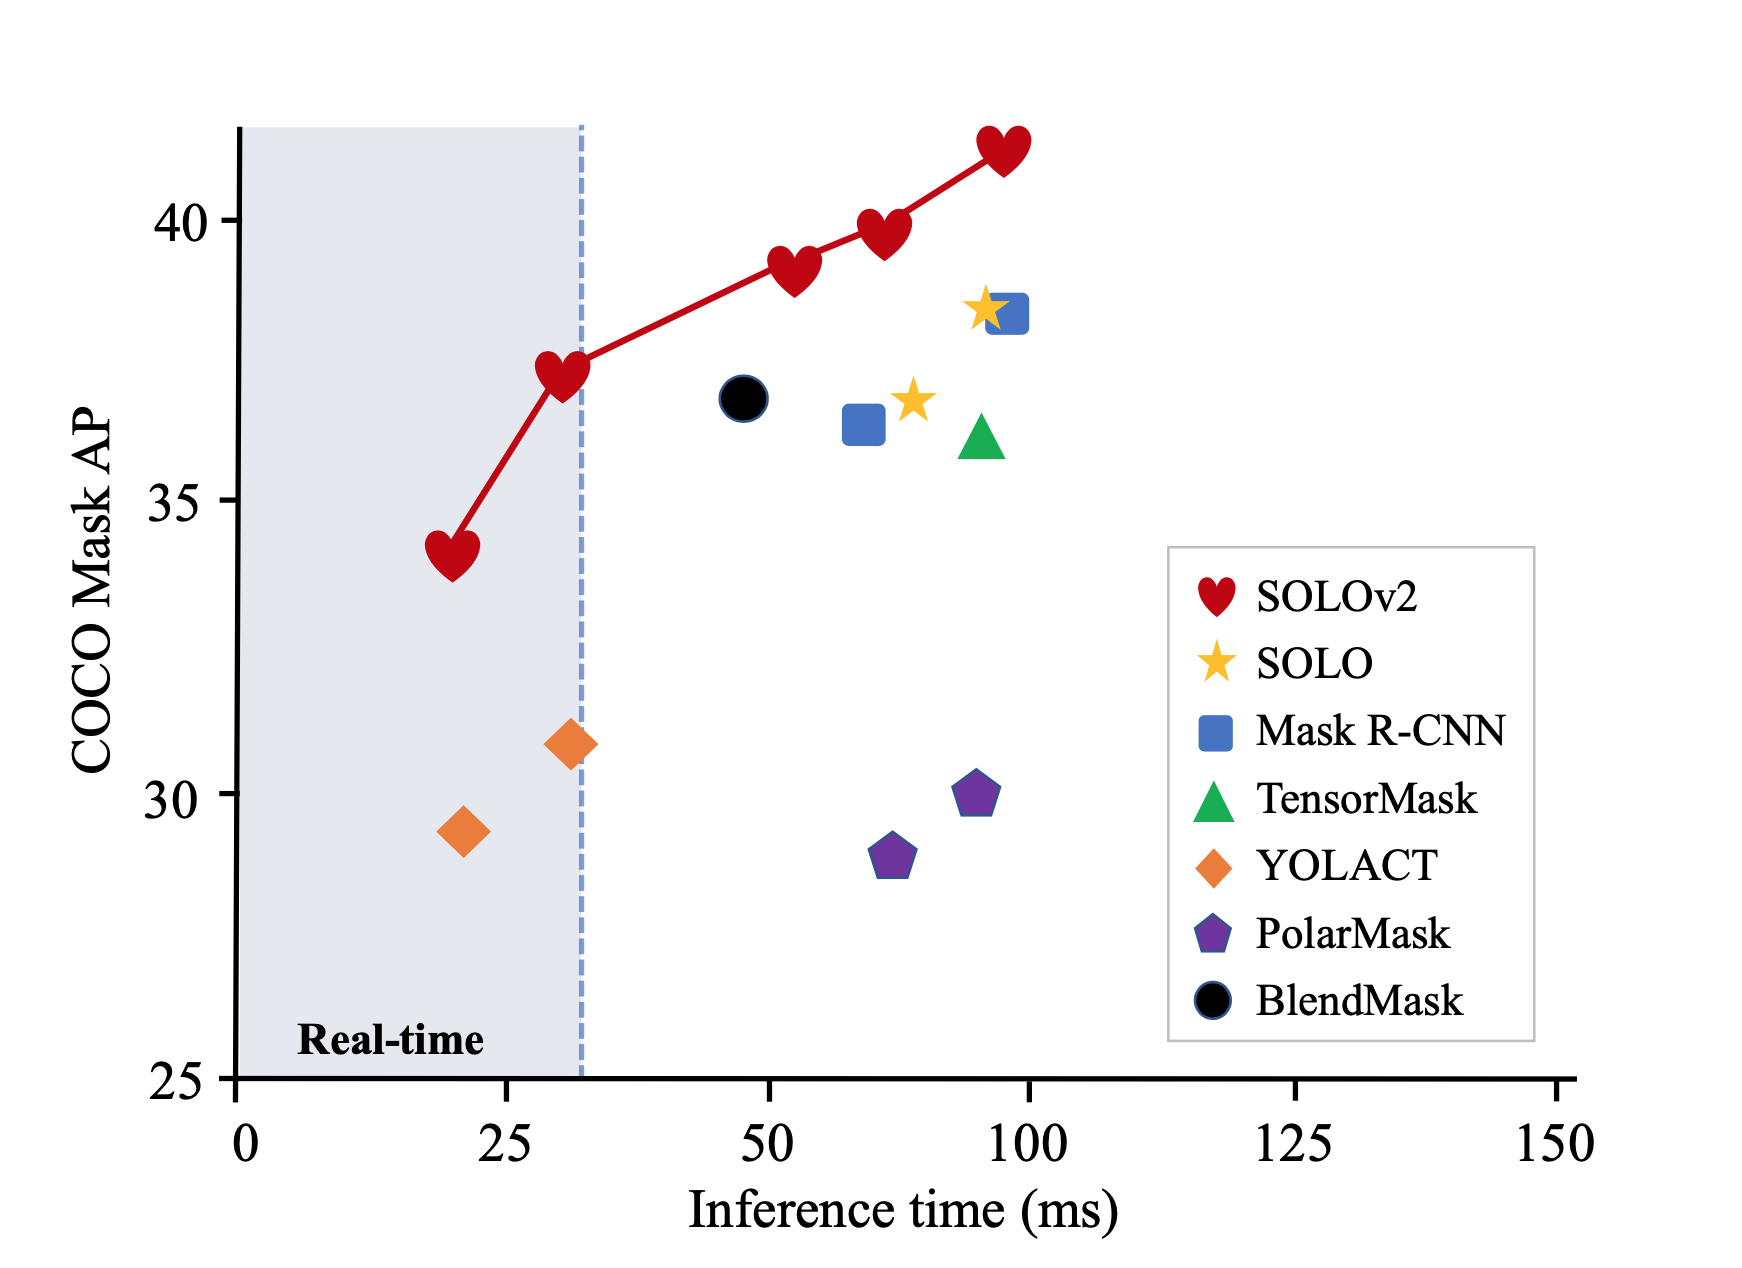
\includegraphics[width=0.7\linewidth]{./image/conclusion_SOLOv2.png}
  \caption{Comparison between SOLOv2 and other stage approches. \textit{Source:~\cite{Authors6_SOLOv2}, pag. 2.}\\ From top to bottom: SOLOv2\cite{Authors6_SOLOv2} and SOLO\cite{solo} are box-free one-stage approch; Mask R-CNN is box-based two-stage approch; TensorMask~\cite{tensormask} is dense sliding-window one-stage approch; YOLACT~\cite{yolact} is one-stage approch predecessor of \textit{BlendMask}~\cite{Authors2_BlendMask}; PolarMask~\cite{polarmask} anchor box-free, single shot instance segmentation one-stage approch; BlendMask~\cite{Authors2_BlendMask} anchor box-free one-stage approch.}
  \label{fig:conclusionSOLOv2}
\noindent
\end{figure}
Moreover, stage approaches are not the only possible methods for solving instance segmentation tasks.
For example, there is Deep Snake~\cite{Authors7_deepsnake}, a counter based approach that outperforms Mask R-CNN~\cite{Authors1_maskrcnn} both in terms of inference speed and AP precision, as shown by the table in Figure \ref{fig:conclusiondeepsnake}, and has the potential to be a good competitor to SOLOv2~\cite{Authors6_SOLOv2}.
%Inoltre gli stage approch non sono gli unici metodi possibili per risolvere tasks di istance segmentation. Per esempio esiste Deep Snake~\cite{Authors7_deepsnake}, counter based approch che supera Mask R-CNN~\cite{Authors1_maskrcnn} sia in termini di velocit\`a di inferenza che AP precision, come mostrato dalla nella tablella in Figure \ref{fig:conclusiondeepsnake}, e ha il potenziale per essere un buon competitor di SOLOv2~\cite{Authors6_SOLOv2}. 
\begin{figure}[H]
\centering
  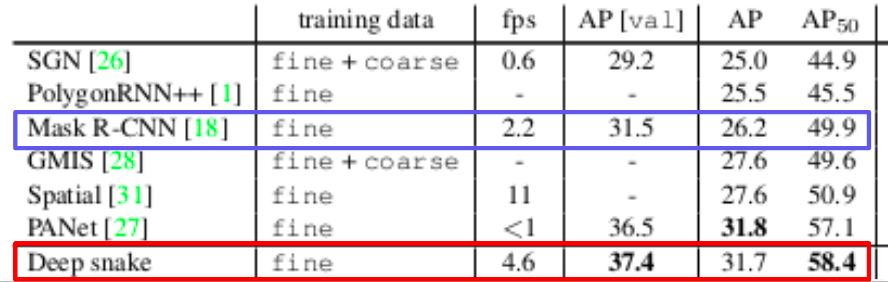
\includegraphics[width=1\linewidth]{./image/conclusion_deepsnake.png}
  \caption{Results on \textit{Cityscapes} val (AP [val] column) and test (remaining columns) sets. \textit{Source:~\cite{Authors7_deepsnake}, pag. 7.}}
  \label{fig:conclusiondeepsnake}
\noindent
\end{figure}
A possible future extension, in line with the results and considerations we have made, could consist in search to further improve the performance of BlendMask~\cite{Authors2_BlendMask} by trying to use Deep Snake~\cite{Authors7_deepsnake} contour-based approach for detecting object bounding boxes of a image.
%Una possibile estensione futura, in linea con i risultati e le considerazioni che abbiamo fatto, potrebbe consistere nel cercare di migliorare ulteriormente le performance di BlendMask, provando a utilizzare l'approccio basato su contorni, di Deep Snake, per il rilevamento dei riquadri di delimitazione degli oggetti di un immagine.

\begin{thebibliography}{1}
\bibitem{Authors1_maskrcnn}
Kaiming He and Georgia Gkioxari and Piotr Dollár and Ross Girshick.
Mask R-CNN. CoRR, 2018.
\bibitem{Authors2_BlendMask}
Hao Chen, Kunyang Sun, Zhi Tian, Chunhua Shen, Yongming Huang and Youliang Yan.
BlendMask: Top-Down Meets Bottom-Up for Instance Segmentation. CoRR, 2020.
\bibitem{Authors3_MSCOCO}
Tsung-Yi Lin, Michael Maire, Serge J. Belongie, Lubomir D. Bourdev, Ross B. Girshick, James Hays, Pietro Perona, Deva Ramanan, Piotr Doll\'ar and C. Lawrence Zitnick.
Microsoft COCO: Common Objects in Context. CoRR, 2014.
\bibitem{Authors4_LVIS}
Agrim Gupta, Piotr Doll\'ar and Ross B. Girshick.
LVIS: A Dataset for Large Vocabulary Instance Segmentation. CoRR, 2019.
\bibitem{cityscapes}
Marius Cordts, Mohamed Omran, Sebastian Ramos, Timo Rehfeld, Markus Enzweiler, Rodrigo Benenson, Uwe Franke, Stefan Roth and Bernt Schiele.
The Cityscapes Dataset for Semantic Urban Scene Understanding. CoRR, 2016.
\bibitem{wildDash}
Zendel, Oliver and Honauer, Katrin and Murschitz, Markus and Steininger, Daniel and Dominguez, Gustavo Fernandez.
WildDash - Creating Hazard-Aware Benchmarks. Proceedings of the European Conference on Computer Vision, (ECCV), 2018.
\bibitem{Authors5_ResNet}
Kaiming He, Xiangyu Zhang, Shaoqing Ren and Jian Sun.
Deep Residual Learning for Image Recognition. CoRR, 2015.
\bibitem{Authors6_SOLOv2}
Xinlong Wang,Rufeng Zhang,Tao Kong, Lei Li and Chunhua Shen.
SOLOv2: Dynamic, Faster and Stronger. CoRR, 2020.
\bibitem{Authors7_deepsnake}
Sida Peng, Wen Jiang, Huaijin Pi, Hujun Bao and Xiaowei Zhou.
Deep Snake for Real-Time Instance Segmentation. CoRR, 2020.
\bibitem{fasterRCNN}
Shaoqing Ren, Kaiming He, Ross B. Girshick, Jian Sun.
Faster R-CNN: Towards Real-Time Object Detection with Region Proposal Networks. CoRR, 2015.
\bibitem{fig1}
Bienias, Lukasz \& n, Juanjo \& Nielsen, Line \& Alstrøm, Tommy. Insights Into The Behaviour Of Multi-Task Deep Neural Networks For Medical Image Segmentation. 2019.
\bibitem{FPN}
Tsung-Yi Lin, Piotr Doll\'ar, Ross B. Girshick, Kaiming He, Bharath Hariharan and Serge J. Belongie.
Feature Pyramid Networks for Object Detection. CoRR, 2016.
\bibitem{fcos}
Zhi Tian, Chunhua Shen, Hao Chen and Tong He.
FCOS: Fully Convolutional One-Stage Object Detection. CoRR, 2019.
\bibitem{solo}
Xinlong Wang, Tao Kong, Chunhua Shen, Yuning Jiang and Lei Li
SOLO: Segmenting Objects by Locations. CoRR, 2019.
\bibitem{imagenet}
J. Deng, W. Dong, R. Socher, L. -J. Li, Kai Li and Li Fei-Fei.
"ImageNet: A large-scale hierarchical image database," 2009 IEEE Conference on Computer Vision and Pattern Recognition, 2009, pp. 248-255, doi: 10.1109/CVPR.2009.5206848.
\bibitem{resnet101_img}
Chen, Jiayao \& Zhou, Mingliang \& Zhang, Dongming \& Huang, H. \& Zhang, Fengshou. (2021).
Quantification of water inflow in rock tunnel faces via convolutional neural network approach. Automation in Construction. 123. 103526. 10.1016/j.autcon.2020.103526. 
\bibitem{resxt}
Saining Xie, Ross B. Girshick, Piotr Doll\'ar, Zhuowen Tu and Kaiming He.
Aggregated Residual Transformations for Deep Neural Networks. CoRR, 2016.
\bibitem{deeplab}
Liang-Chieh Chen, Yukun Zhu, George Papandreou, Florian Schroff and Hartwig Adam.
Encoder-Decoder with Atrous Separable Convolution for Semantic Image Segmentation. CoRR, 2018.
\bibitem{protonet}
Daniel Bolya, Chong Zhou, Fanyi Xiao and Yong Jae Lee.
YOLACT: Real-time Instance Segmentation. CoRR, 2019.
\bibitem{Authors8_semanticloss}
Xu, Jingyi and Zhang, Zilu and Friedman, Tal and Liang, Yitao and Van den Broeck, Guy.
A Semantic Loss Function for Deep Learning with Symbolic Knowledge. Proceedings of the 35th International Conference on Machine Learning, 2018.
\bibitem{tensormask}
Xinlei Chen, Ross B. Girshick, Kaiming He and Piotr Doll\'ar.
TensorMask: A Foundation for Dense Object Segmentation. CoRR, 2019.
\bibitem{yolact}
Daniel Bolya, Chong Zhou, Fanyi Xiao and Yong Jae Lee.
YOLACT: Real-time Instance Segmentation. CoRR, 2019.
\bibitem{polarmask}
Enze Xie, Peize Sun, Xiaoge Song, Wenhai Wang, Xuebo Liu, Ding Liang, Chunhua Shen and Ping Luo.
PolarMask: Single Shot Instance Segmentation with Polar Representation. CoRR, 2019.

\end{thebibliography}



\end{document}
